\chapter{UCN Production and Detection\label{chap:UCNresult}}

In November~2017 the first UCN at TRIUMF were produced via the
prototype vertical UCN source described in
Section~\ref{sec:vertical_source}. Here the spallation neutrons are
converted to UCN through phonon excitation in the isotopically pure
superfluid helium. Several experiments were performed with the UCN
including UCN yield measurements, UCN storage lifetime measurements
and steady-state UCN production. These experiments are essential for
the better understanding of the vertical source and to design the next
generation high intensity UCN source. In this chapter those
experiments are described and the result of the data analysis is
presented.

\section{UCN Cycle of Measurement}
Fig.~\ref{fig:volume_schematic} is a simple schematic of the UCN
production and detection volumes. Here volume $V_1$ is the production
and storage volume before the valve where $N_1$ number of UCN are
produced, $V_2$ is the secondary volume where $N_2$ number of UCN
could enter after the valve is opened, and $V_3$ is the detector
volume where $N_3$ number of UCN could reach the detector.



\begin{figure}[h]
  \centering
  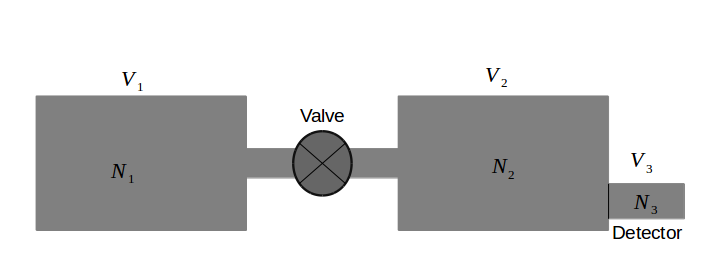
\includegraphics[width=0.9\textwidth]{volume_schematic.png}
  \caption{Schematic drawing of a simple UCN source. $V_1$ is the
    production volume with $N_1$ number of UCN, $V_2$ is the secondary
    volume where $N_2$ number of UCN exist and $V_3$ is the detector
    with $N_3$ number of UCN. }
  \label{fig:volume_schematic}
\end{figure}

At $t = 0$ when the beam is on and the valve is closed, the number of UCN in
$V_1$ goes up while the total number of UCN in $V_2$ and $V_3$ is
zero. This is described as 

\begin{equation}
  \label{eqn:dndt}
\frac{dN_1}{dt} = P - \frac{N_1}{\tau_1}  
\end{equation}
where $P$ is the UCN production rate in the source as describe in
Section~\ref{sec:UCN_production} and $\tau_1$ is the UCN storage
lifetime in the source.  After the beam is turned off, the valve is
opened and the UCN could travel to the volume $V_2$ and eventually
$V_3$. The valve is usually left open for 2 to 3 minutes in the
measurements with the vertical source. The UCN trade between $V_1$,
$V_2$ and $V_3$ is described by the differential
Eqn.~\ref{eqn:alldndt}.

\begin{equation}
  \label{eqn:alldndt}
  \begin{aligned}
    \frac{dN_1}{dt} =&- \frac{N_1}{\tau_{c,1}} - \frac{N_1}{\tau_1} + \frac{N_2}{\tau_{c,2}}  \\
    \frac{dN_2}{dt} =& \frac{N_1}{\tau_{c,1}} - \frac{N_2}{\tau_{c,2}} - \frac{N_2}{\tau_2} - \frac{N_2}{\tau_{c,3}} \\
    \frac{dN_3}{dt} =& \frac{N_2}{\tau_{c,3}}.
  \end{aligned}
\end{equation}


In these equations, \large $\frac{dN_1}{dt}$ \normalsize shows the
change in the UCN counts over time in $V_1$,~\large $\frac{dN_2}{dt}$
\normalsize shows the change in the UCN counts in $V_2$ and \large
$\frac{dN_3}{dt}$ \normalsize shows the change in the UCN count in $V_3$
which is the detector after the valve is opened. Each term is described below.

The total number of UCN in $V_1$ depends on three factors. The UCN that
get into $V_2$~\large($\frac{N_1}{\tau_{c,1}}$) \normalsize, the UCN that is lost
with the storage lifetime of $\tau_1$, and the UCN that bounce back from
$V_2$ to $V_1$~\large ($\frac{N_2}{\tau_{c,2}}$) \normalsize.
In $V_2$, some UCN cross from $V_1$ to $V_2$~ \large
($\frac{N_1}{\tau_{c,1}}$) \normalsize, some get lost with the
lifetime of $\tau_2$~\large ($\frac{N_2}{\tau_2}$) \normalsize, some
cross the gate valve and go back to $V_1$~ \large
($\frac{N_2}{\tau_{c,2}}$)\normalsize and some get to the detector
~\large ($\frac{N_2}{\tau_{c,3}}$) \normalsize. The rate of the UCN
detection $\frac{dN_3}{dt}$ is the number of UCN crossing from $V_2$.
Solving these equation could give an estimate of the UCN rate.

A 3D drawing of the experimental setup is shown in
Fig.~\ref{fig:Source_all}. In this case, $V_1$ is the UCN source
bottle and the horizontal section of the UCN guide before the UCN gate
valve and $V_2$ and $V_3$ are the volumes after the UCN valve and the
detector volume respectively.

\begin{figure}[h!]
  \centering
  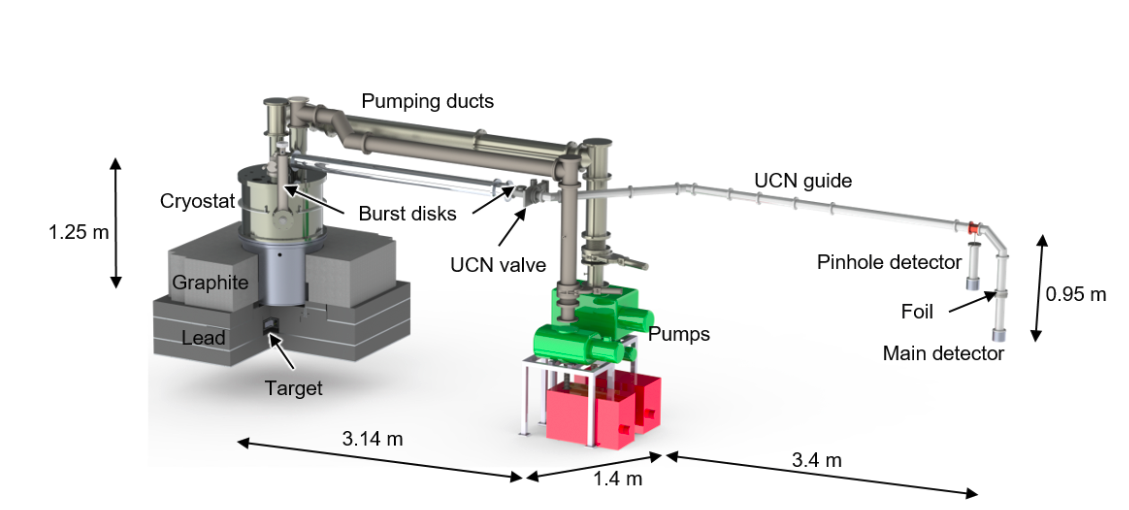
\includegraphics[width=1.1\textwidth]{Source_all.png}
  \caption{The UCN source and the guide geometry at TRIUMF }
  \label{fig:Source_all}
\end{figure}
The process of UCN production described above is refered to the UCN
production in the {\it {batch mode}} since the UCN is accumulated in
the source while the UCN valve is left close. Here the target is
irradiated and the UCN are produced in the source. After the
irradiation stops, the UCN valve is opened and UCN could bounce of the
guide walls and reach the detector volume. In the standard UCN
production measurements, the applied beam current is 1~$\mu$A and the
target is irradiated for 60~s. One cycle of measurement is shown in
Fig.~\ref{fig:UCNRate}. The UCN valve is typically left open for 2
minutes. The end of a UCN cycle is defined by the UCN valve close
time. Once the UCN valve is closed, a new cycle of measurement starts.


\begin{figure}[h!]
  \centering
  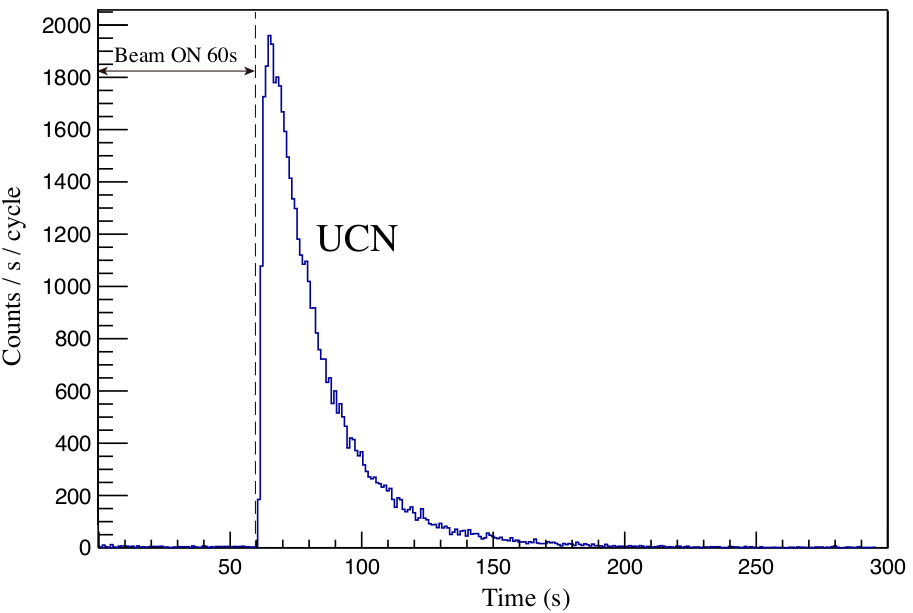
\includegraphics[width=0.8\textwidth]{UCNRate.png}
  \caption{The figure shows the UCN rate at 60~s irradiation time and
    1~$\mu$A beam current. In this case, the UCN gate valve is opened
    immediately after the end of irradiation. At this time, the UCN
    rate reaches the peak of about 2000 UCN/s. The UCN rate decays
    down to the background noise. The Valve is left open for 120~s. }
  \label{fig:UCNRate}
\end{figure}


Another possible mode of operation is when we leave the UCN valve open
while irradiating the target. This is called the {\it{ steady-state}}
mode where we have a constant stream of UCN to the main detector~(see
Section~\ref{sec:steadystate}).

The following sections are focused on the result of the UCN yield
optimization, the UCN storage lifetime measurements, UCN production in
the steady-state mode and the comparison of those measurements with
simulations.


\section {Data Quality Checks}
The main detector for most of the experiments is the $^6\mathrm{Li}$
glass based scintillator detector which was described in
Section~\ref{sec:Li6detector}. Before using the collected data to
extract the desired information, it is critical to make sure that the
detector was working as expected and the data is reliable. Here some
data quality checks are reported.


The PSD versus $Q_L$ distribution from a UCN data run is shown in
Fig.~\ref{fig:psd_vs_ql} for all the PMTs combined. This is the most useful
way of separating the signal and background.
% The graph is for run 541
\begin{figure}[h!]
  \centering
  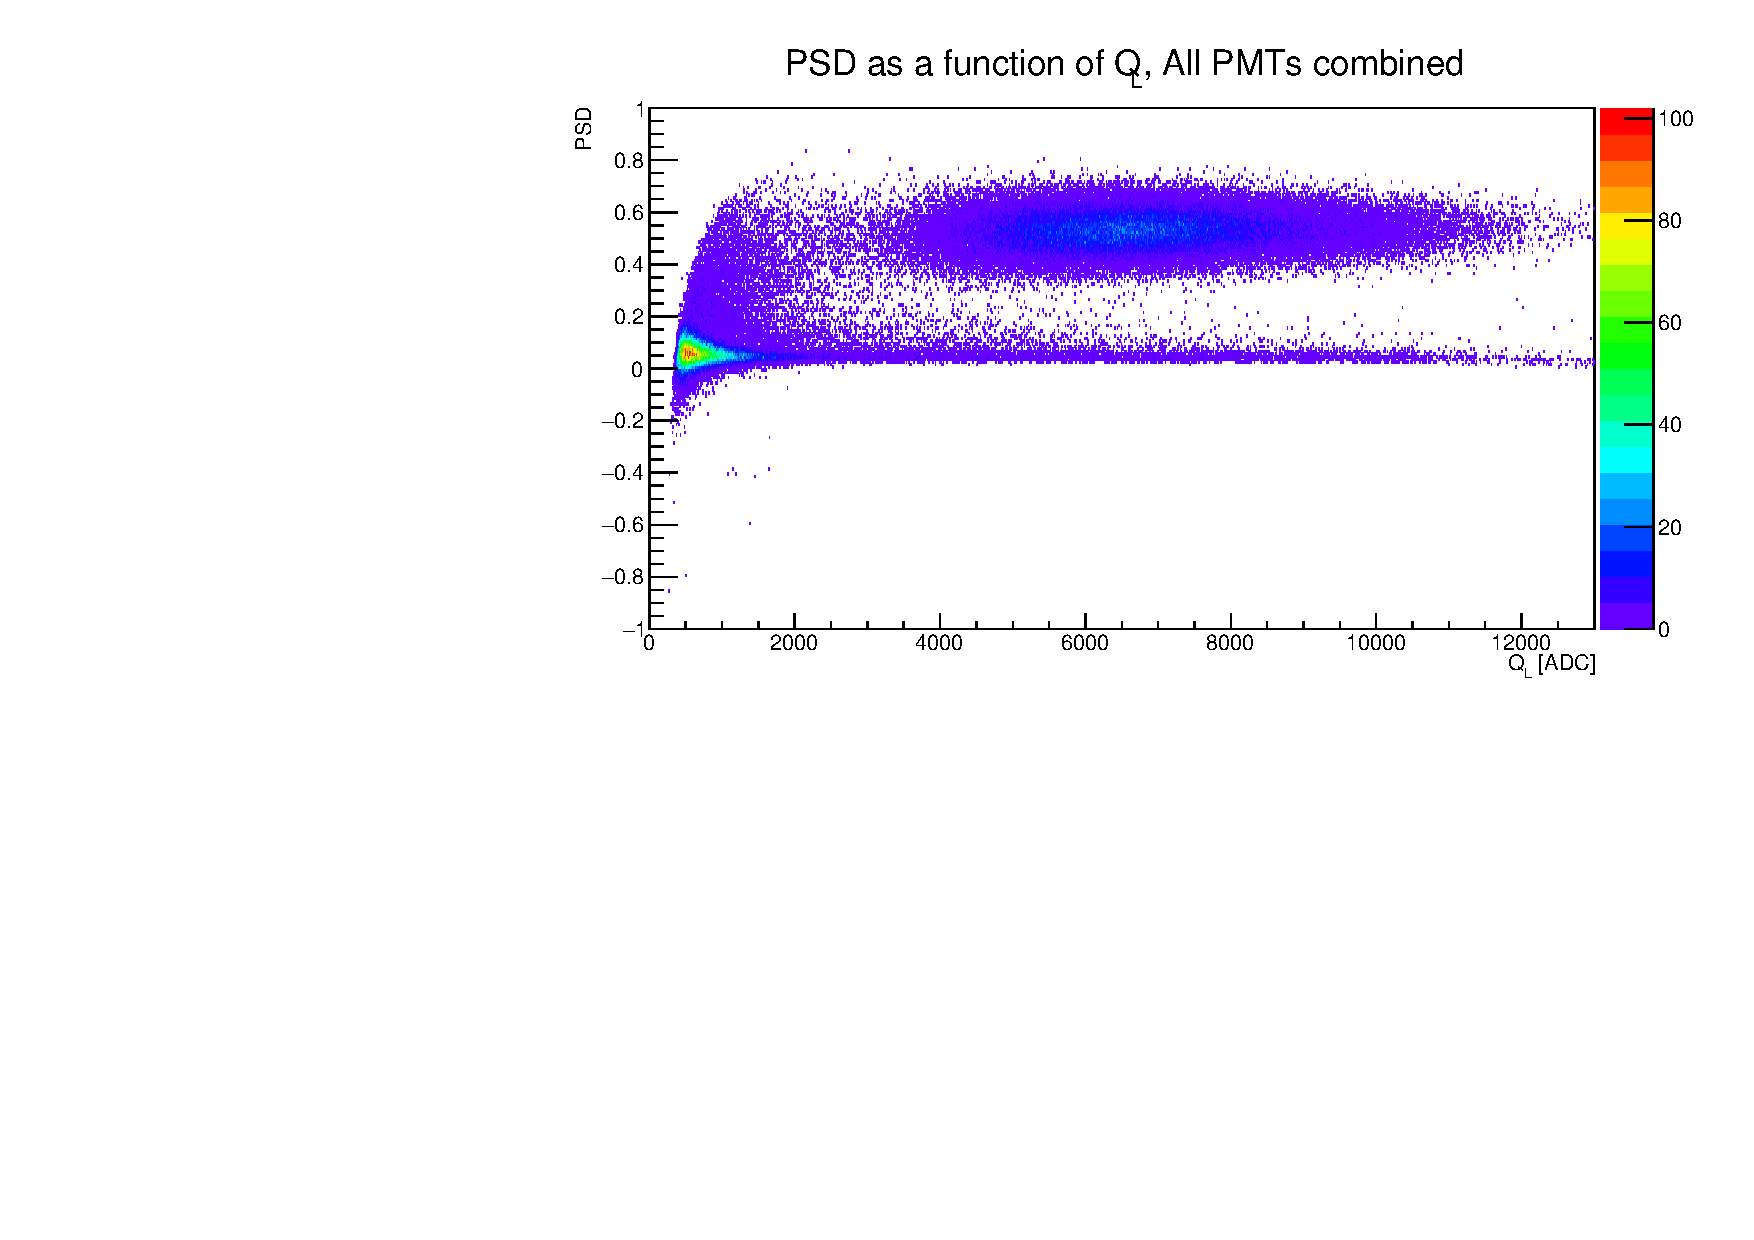
\includegraphics[width=0.9\textwidth]{PSD_vs_QL.pdf}
  \caption{PSD versus $Q_L$ for all of the PMTs for a standard
    1~$\mu$A proton beam current and 60~s target irradiation time }
  \label{fig:psd_vs_ql}
\end{figure}
Here the UCN events are mainly around the PSD value of 0.5 and $Q_L$
between 3000 and 12000. The events at PSD~$\sim 0$ represent the
$\gamma$-rays in the lightguides. To get the actual UCN counts, a PSD
cut of 0.3 and a $Q_L$ cut of 2000 were applied. This ensures that
only the UCN events are counted represented by the central oval-shaped
region. Out of all 9 channels, the centeral channel counts the most
number of UCN events while the corner channels receive the least as
expected. Fig.~\ref{fig:channelcounts}.

\begin{figure}[h!]
  \centering
  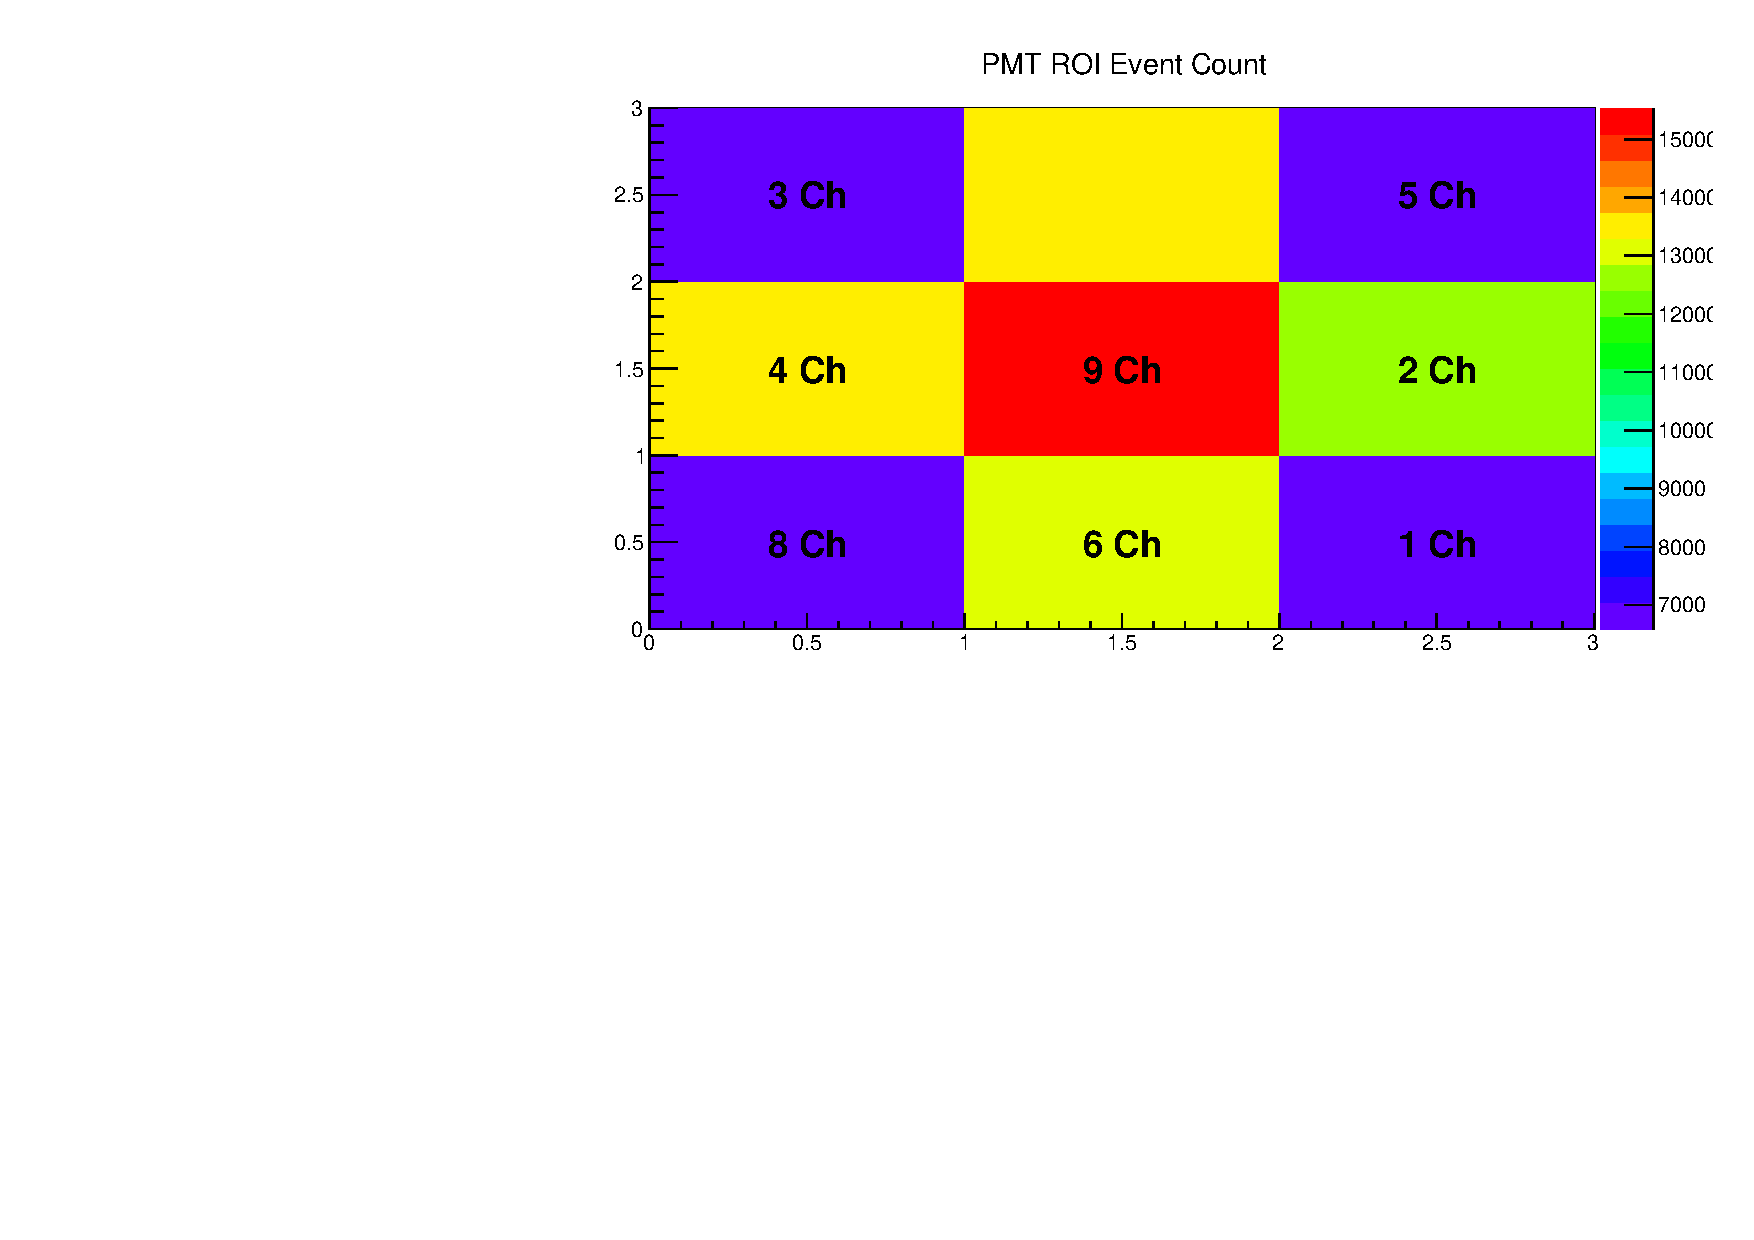
\includegraphics[width=0.9\textwidth]{channelcounts.pdf}
  \caption{Number of UCN events for each channel. The total number of
    UCN events decrease as we move towards the corner channels.  }
  \label{fig:channelcounts}
\end{figure}


The effect of the detector on the UCN counts could be categorized in
three groups: Deadtime, Crosstalk and Pileup. Deadtime is the minimum
time difference between two subsequent UCN events in the same PMT
which might give rise to loss in the UCN counts. Crosstalk is the
multiple trigger events in neighboring PMTs originated from the same
UCN events. This effect might increase the possiblitiy of
overestimating the total UCN counts. Pileup is the combination of
multiple events into a single event. It includes UCN-UCN,
UCN-$\gamma$, $\gamma$-UCN and $\gamma$-$\gamma$ pileups. The true
number of UCN counts is estimated as
\begin{equation}
  \label{eqn:trueUCN}
  N^{\mathrm{True}}_{\mathrm{UCN}} = \left [ N^{\mathrm{raw}}_{\mathrm{UCN}} \cdot \left( 1 + \alpha_{pl} + \alpha_{ct}\right) \right] \cdot A_{box}
\end{equation}
where $\alpha_{pl}$ is the estimated pileup coefficient from data and
independant calculations assuming Poisson statistics, $\alpha_{ct}$ is
the estimated time-coincidence analysis on data and $A_{box}$ is the
UCN box efficiency estimated using Monte-Carlo simulations. Based on
our Monte-Carlo simulations the $\gamma$-UCN and UCN-$\gamma$ pileups
are not a concern for UCN counting. In addition, $\gamma$-$\gamma$
pileup does not leak into the UCN box.

The result of such analyses showed that the UCN box acceptance is at
97. $\pm$ 0.1~\%. The UCN-UCN pileup at 1~$\mu$A beam current and 60~s
irradiation of the target was measured to be at 0.075~Hz or has and
effect of less than 1~\%. The analysis showed very little evidence for
cross-talk and less than 2~\% deadtime effect.



\section{UCN Count Measurement \label{UCNCounts}}

The total number of produced UCN in the vertical source, $N$, at a
certain time t$_i$ when the UCN valve is closed is the integration of
eqn.~\ref{eqn:dndt}
\begin{equation}
  \label{eq:totalUCN}
  N = P \tau_1\left[ 1- \exp \left(\frac{t_i }{ \tau_1}\right) \right]
\end{equation}
where the UCN storage lifetime $\tau_1$ is given by

\begin{equation}
  \label{eqn:tau1}
  \frac{1}{\tau_1} = \frac{ f_1}{\tau_\mathrm{He}} + \frac{1-f_1}{\tau_\mathrm{vapour}}+\frac{1}{\tau_\mathrm{wall,1}} + \frac{1}{\tau_\beta}.
\end{equation}
The storage lifetime consists of four terms: the loss rate in the
superfluid helium $ f_1\tau_\mathrm{He}^{-1}$, the loss rate in the
helium vapour $(1-f_1)\tau_\mathrm{vapour}^{-1}$, the loss rate in the
UCN guide walls $\tau_\mathrm{wall,1}^{-1}$ and the neutron $\beta$
decay $\tau_\beta^{-1}$. The volume in which the UCN are produced
consists of the UCN bottle as well as the horizontal guide section
before the UCN valve~(see Fig.~\ref{fig:Source_all}). This volume is
not fully filled with the superfluid helium. As a result, $ f_1$ is
the probablity of UCN being in the superfluid helium while the UCN
valve is closed. After the valve is opened, the total UCN lifetime is

\begin{equation}
  \label{eqn:tau2}
  \frac{1}{\tau_2} = \frac{ f_2}{\tau_\mathrm{He}} + \frac{1-f_2}{\tau_\mathrm{vapour}}+ \frac{1}{\tau_\mathrm{wall,2}}+\frac{1}{\tau_d} + \frac{1}{\tau_\beta}
\end{equation}
where $\tau_d^{-1}$ is the loss rate in the detector,
$f_2$ is the probability of UCN being in the superfluid
helium and ${\tau_\mathrm{wall,2}}^{-1}$ is the UCN guide loss rate in
this case where the valve is open and the target irradiation is
stopped. Fig.~\ref{fig:UCNRate_with_lines} shows three measurement
cycles at 1~$\mu$A beam current and 60~s irradiation time with
zero second delay time for opening the UCN valve. The dashed lines
indicate the start of the irradiation for a cycle, the dotted lines
show the end of irradiation which in this case is the same as the UCN
valve open time. The solid lines shows the valve close time.


\begin{figure}[h!]
  \centering
  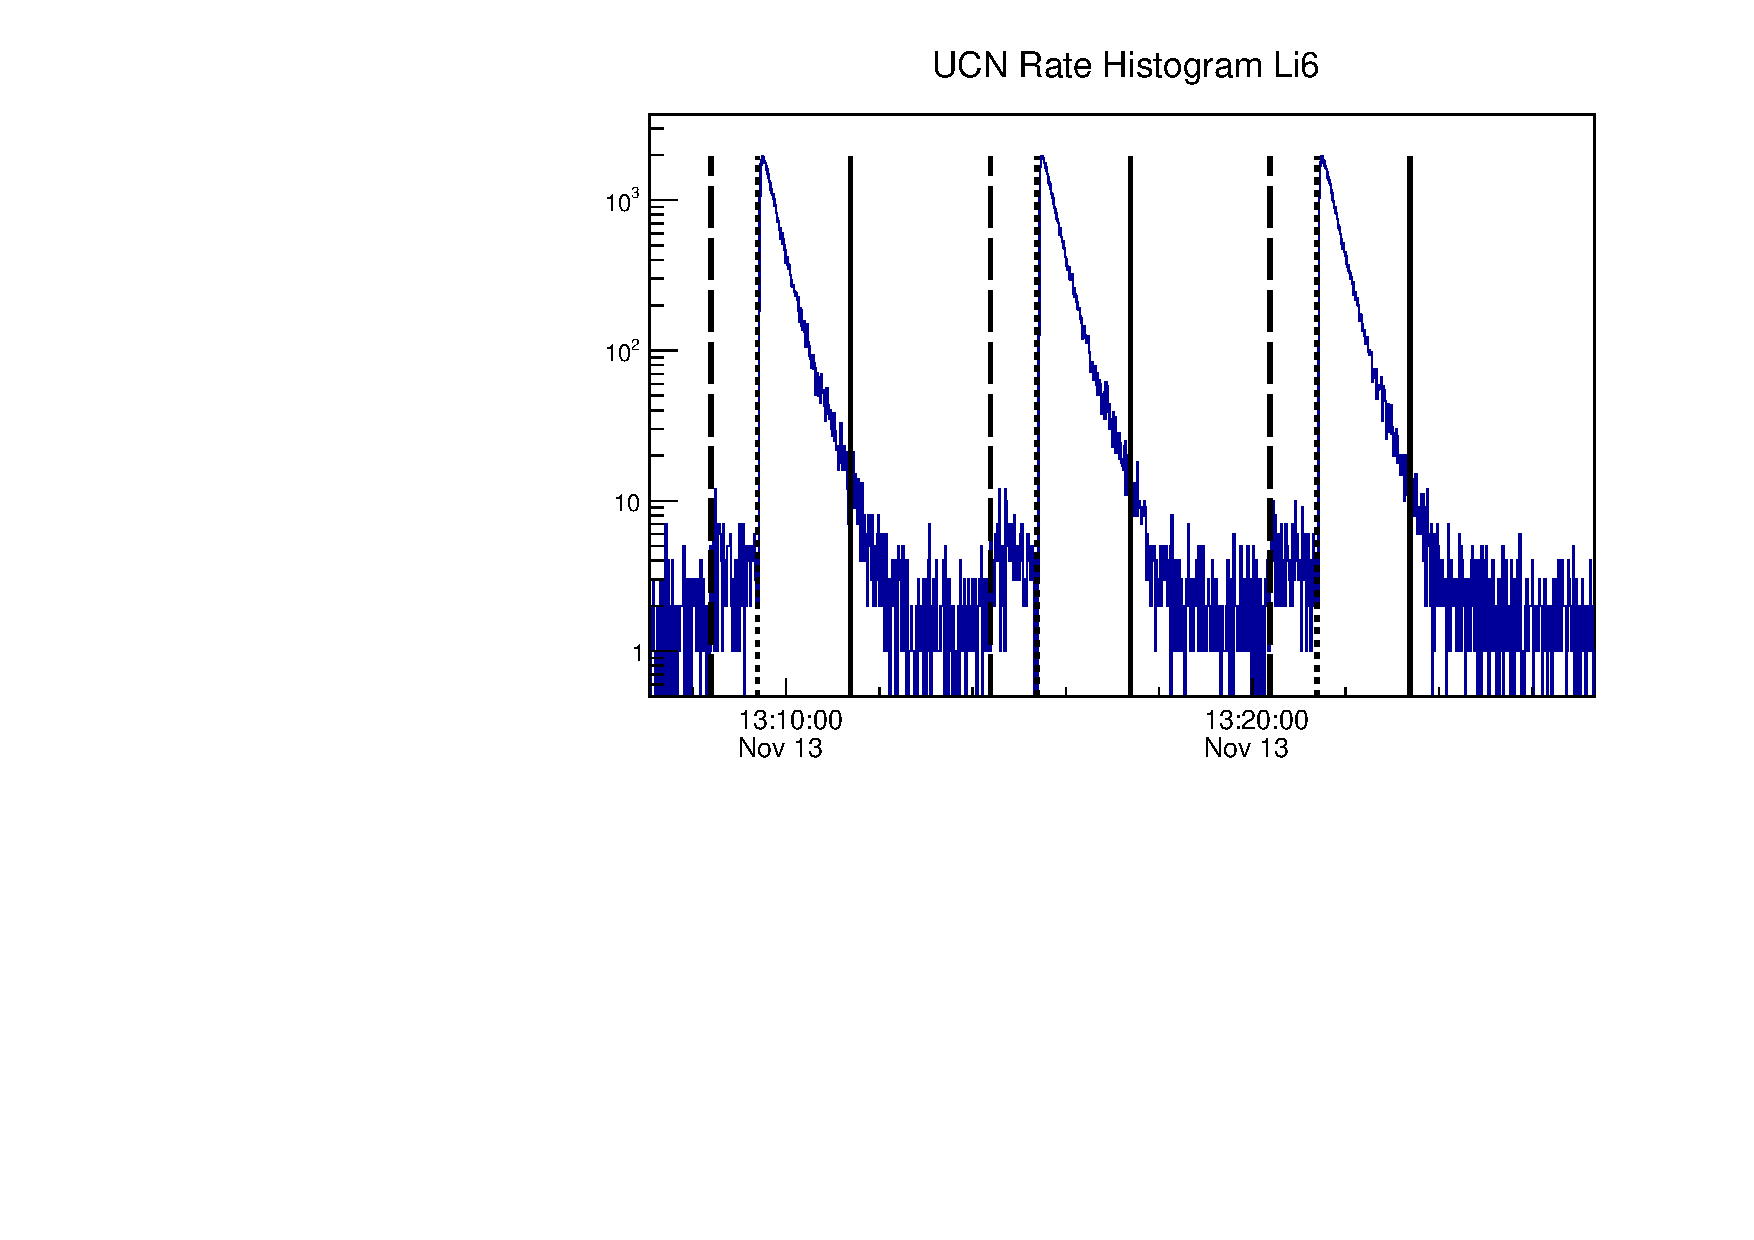
\includegraphics[width=1.0\textwidth]{UCNRate_with_lines_logy.pdf}
  \caption{Three measurement cycles for 1~$\mu$A beam current, 60~s
    irradiation time and 0~s valve open delay time. The dashed lines
    show the start of the target irradiation, the dotted lines show
    the end of the irradiation and the valve open time for each cycle
    and the solid lines show the end of a cycle which is the valve
    close time.}
  \label{fig:UCNRate_with_lines}
\end{figure}

The total UCN counts are given by the integration of all the UCN
events for the duration of the valve open time. However, this method
of counting includes the measured background UCN as well. To subtract
the background counts from the actual UCN counts the UCN background
rate is calculated before the start of the irradiation of that
particular cycle. This rate is then multiplied by the valve open
duration time which then gives an estimate of the total background UCN
counts. The background rate is typically less than 5~UCN/s. The
subtraction of the latter from the total UCN counts gives the actual
UCN counts that are produced by the isopure helium converter and
detected by the detector. At low and moderate UCN counts, the
statistical uncertainty is available by taking the square root of the
number of measured events, as follows conveniently from Poisson
statistics~\cite{pomme2015uncertainty}.
%%%%%%%%%%
\subsection{UCN Yield Versus Proton Beam Current}
The UCN yield at different proton beam currents is also
studied. Fig.~\ref{fig:counts_vs_beam} shows the total UCN counts
versus the applied proton beam current in $\mu$A at 60~s irradiation
time. The background UCN is subtracted off from the detected UCN
counts as explained earlier. At lower beam currents, the total UCN
counts increase linearly with the proton beam current. The dashed line
shows the extrapolation to higher beam currents in an ideal
case. However, at higher beam currents, the total UCN counts deacrese
due to an increase in the heat load on the isotopically pure
superfluid helium and therefore its temperature. Theoretically, the
upscattering rate in the superfluid helium is proportional to its
temperature as $T^7$~(see Section~\ref{sec:upscattering}). This has
been confirmed by performing PENTrack simulations and comparing the
result to the acquired data~(see Section~\ref{sec:pentrack}).



\begin{figure}[h!]
  \centering
  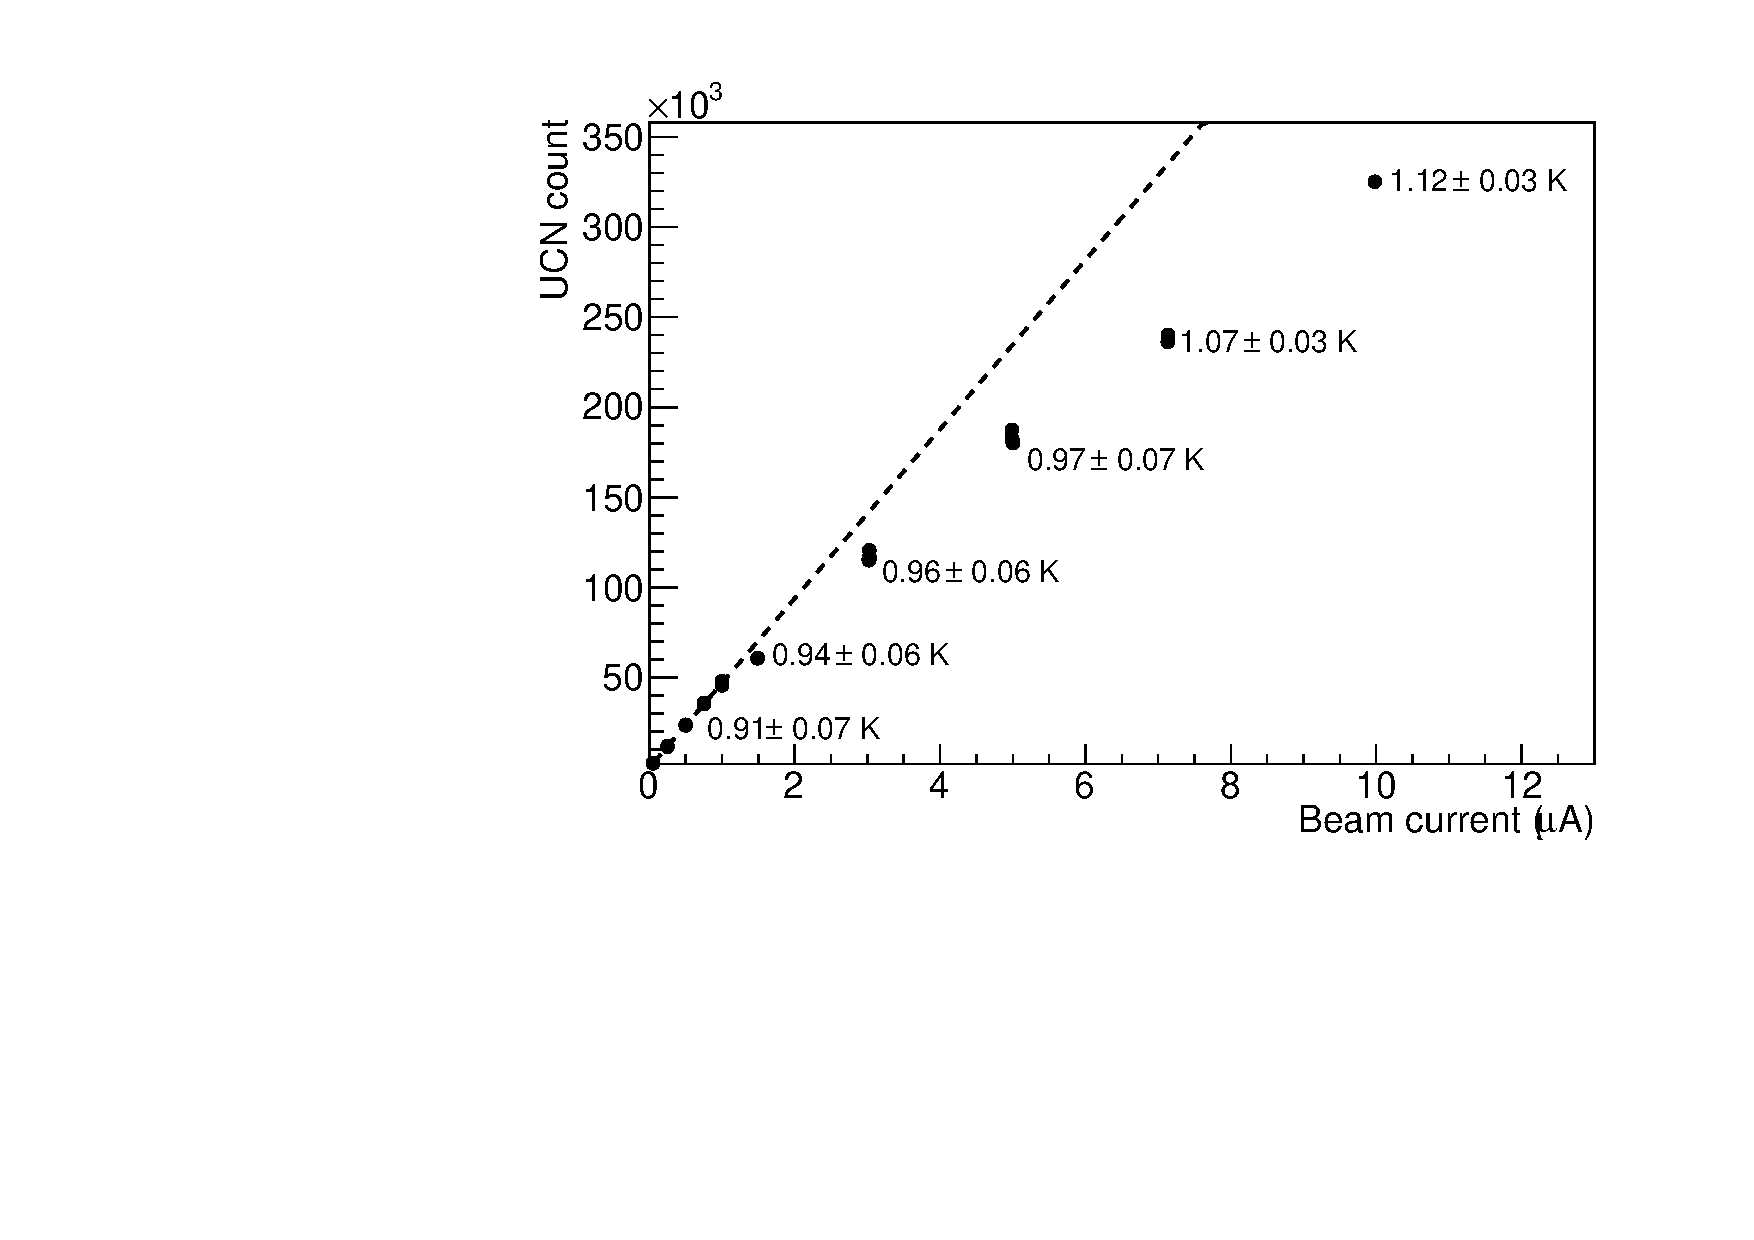
\includegraphics[width=0.8\textwidth]{UCNCounts_vs_Beam.pdf}
  \caption{The total UCN counts versus the applied proton beam
    current. The labelas show the full range of the superfluid helium
    temperature for that measurement. The dashed line is fit to the
    UCN counts at low beam currents.}
  \label{fig:counts_vs_beam}
\end{figure}


The labels in the graph show the full range of the isopure helium
temperatures during the measurement cycle. Four temperature sensors
were used to measure the superfluid helium temperature with the
following names in our EPICS system: TS11, TS12, TS14 and TS16. The
location of these sensors are shown in Fig.~\ref{fig:TSs}. The temperature
sensor TS11 is located at the UCN heat exchanger bottom, the
temperature sensor TS14 is located at the UCN heat exchanger top, the
temperature sensor TS12 is located at the UCN double tube bottom and
the temperature sensor TS16 is located at the UCN double tube top. At
low temperatures around 0.8~K these temperature sensors show a maximum
of 0.1~K discrepancy with TS16 showing the highest value and TS12
showing the lowest value.



\begin{figure}[h!]
  \centering
  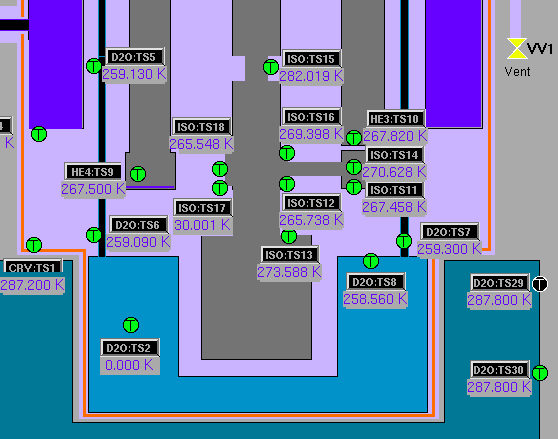
\includegraphics[width=0.8\textwidth]{TSs.png}
  \caption{Zoomed in screenshot of the EPICS temperature monitoring
    screen~\ref{fig:epics}. TS11 is located at the UCN heat exchanger
    bottom, TS12 is located at the UCN double tube bottom, TS14 is
    located at the heat exchanger double tube top and TS16 is located
    at the UCN double tube top. For further information about the
    source schematic see Sec.~\ref{sec:vertical_source} }
  \label{fig:TSs}
\end{figure}

In summary, at lower beam currents, because of the low heat load on the
superfliud helium its temperature change is not significant and it
gives rise to linear increase in the UCN counts versus the applied
proton beam current. However, at higher proton beam currents, the
temperature of the superfluid increases due to higher heat load and it
gives rise to higher upscattering rate in the superfluid and lower UCN
counts.


\subsection{UCN Yield Versus Target Irradiation Times}
The total UCN counts is optimized by irradiating the target at
different proton beam currents and different irradiation times. The
result is shown in Fig.~\ref{fig:counts_vs_irrad}.  In this graph the
vertical axis shows the total number of UCN counts where the
background UCN are subtracted and the horizontal axis shows the target
irradiation times in seconds. Each marker represents a proton beam
current and the dashed line is an exponential fit to those data
points. The proton beam current and the extracted time constant from
the fit are shown in the Figure.

At higher beam currents, the saturation time constant decreases due to
the higher heat load and faster temperature increase in the superfluid
helium. At higher beam currents and longer irradiation times the total
measured UCN counts are below the exponential extrapolation due to the
higher temperature and higher upscattering rate in the superfluid
helium.

\begin{figure}[h!]
  \centering
  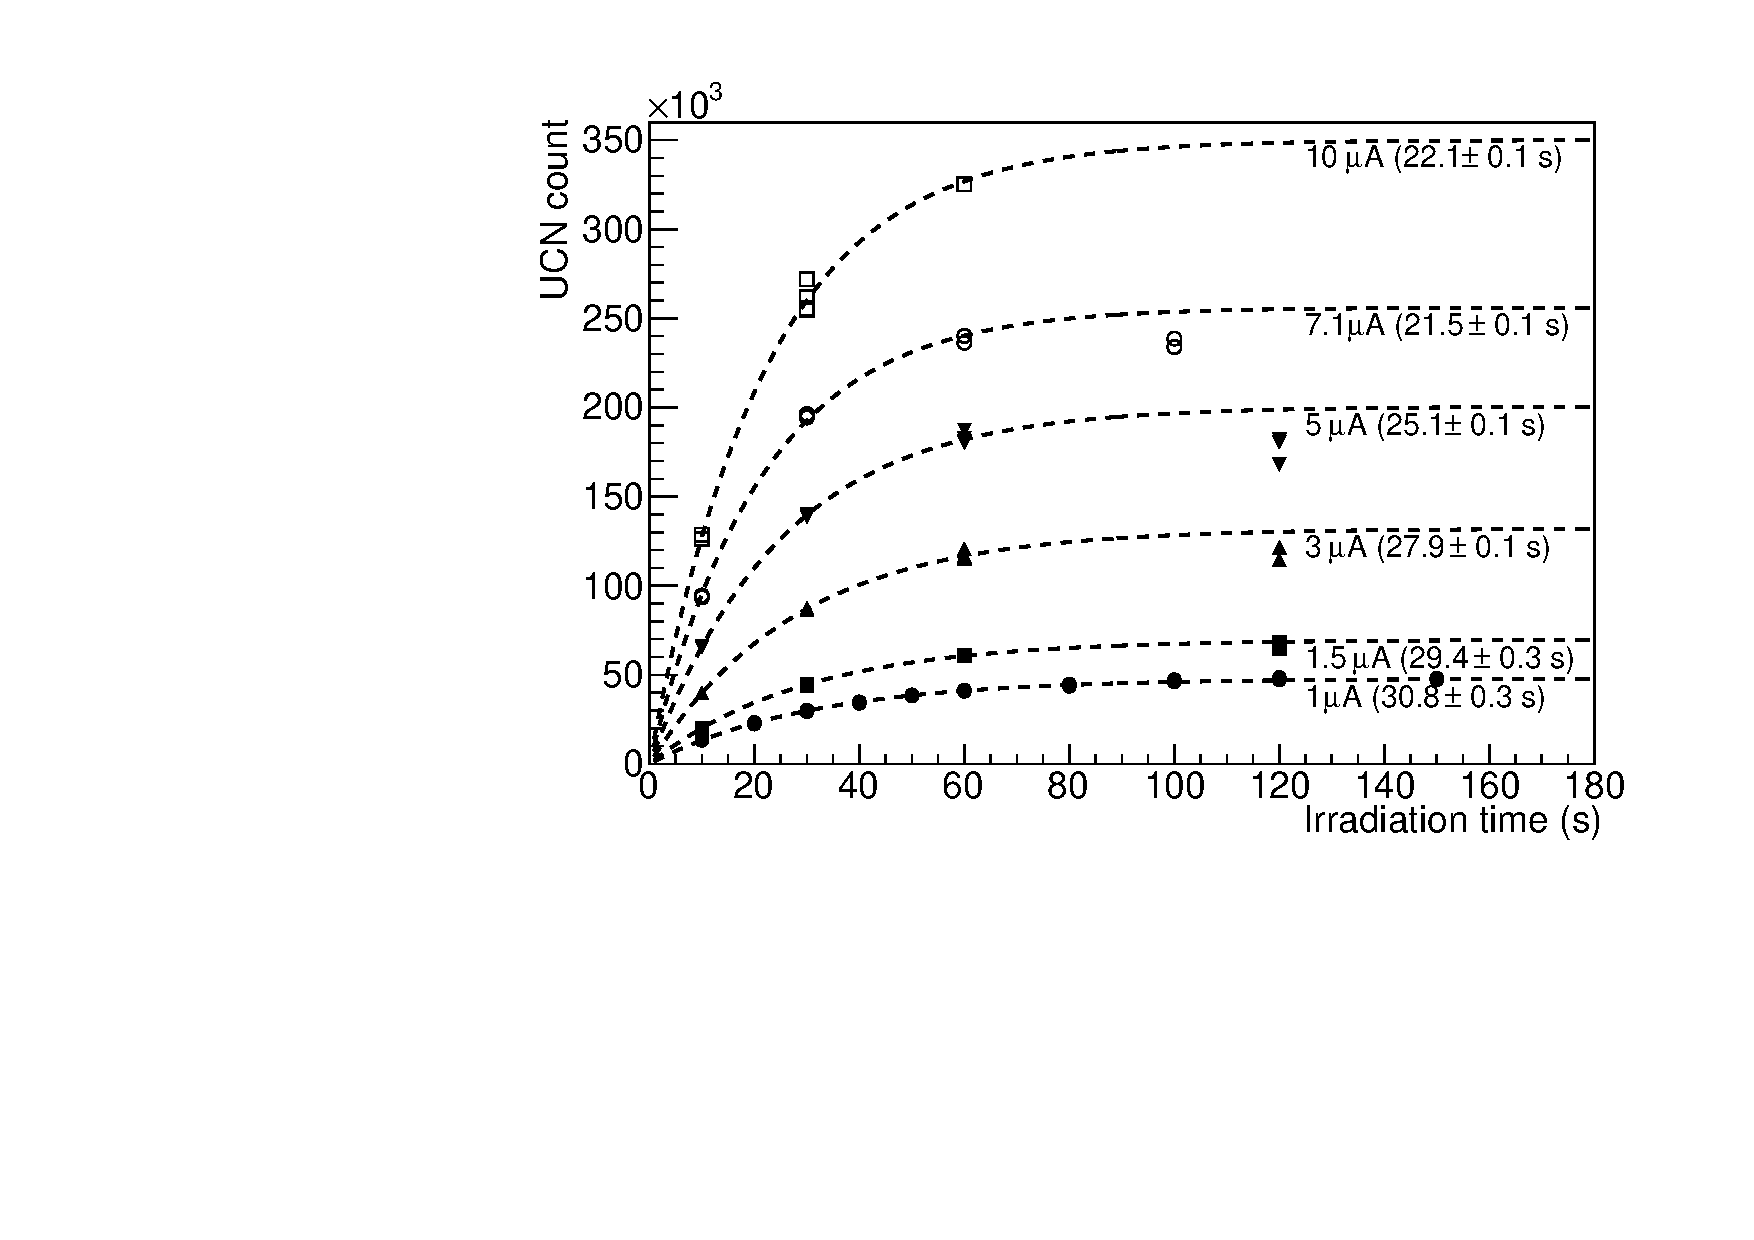
\includegraphics[width=0.8\textwidth]{UCNCounts_vs_irradTime.pdf}
  \caption{Number of UCNs extracted from the source after irradiating
    the target for different times with different beam currents. The
    dashed lines extrapolate the data for irradi- ation times below
    60~s using exponential saturation curves.  The labels show the
    saturation time constant for each beam current. }
  \label{fig:counts_vs_irrad}
\end{figure}


\subsection{UCN Yield Versus Isopure Helium Temperature}
The UCN counts were also measured at different superfluid helium
temperature~(see Fig.~\ref{fig:counts_vs_temp}). The vertical axis
shows the number of UCN counts and the horizontal axis shows the
temperature of the superfluid helium for all four temperature sensors.
The horizontal error bars are calculated as
$(T_{\mathrm{max}}-T_{\mathrm{min}})/2$ for each temperature sensor
where $T_{\mathrm{max}}$ is the maximum value of the superfluid helium
temperature reading by one temperature sensor and $T_{\mathrm{min}}$
is the minimum value read for the same sensor.

\begin{figure}[h!]
  \centering
  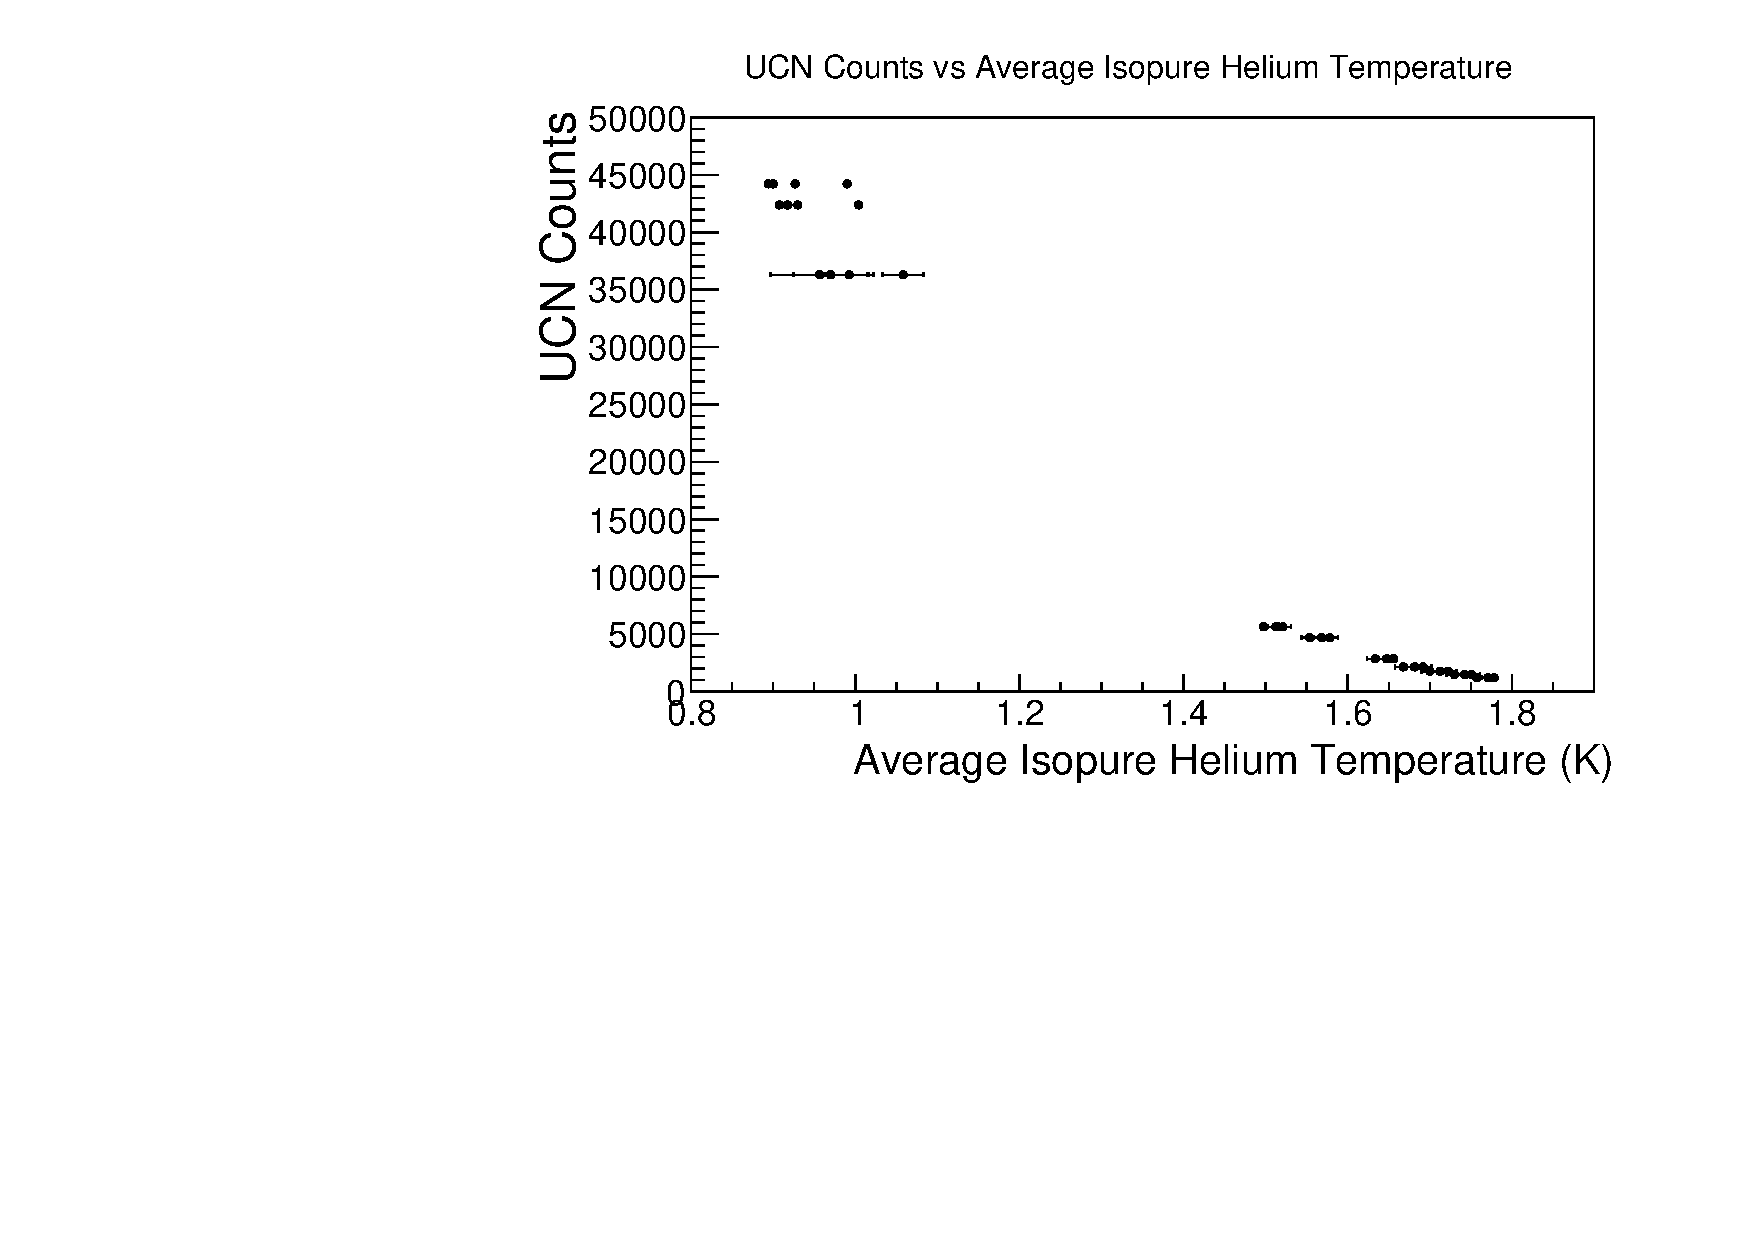
\includegraphics[width=0.9\textwidth]{counts_vs_temp.pdf}
  \caption{UCN yield versus the superfluid helium temperature. At a
    particular UCN ounts, there are several values for the temperature
    of superfluid helium. It is due to the discrepancy in the
    temperature sensor readings.}
  \label{fig:counts_vs_temp}
\end{figure}

As the temperature of the superfluid helium increases, the
number of UCN counts in the detector decreases as expected. This is
mainly due to the high UCN upscattering rate in the superfluid helium
at higher temperatures.


\subsection{Steady-state UCN Production\label{sec:steadystate}}

The result shown so far are achieved in the batch mode of
operation. In addition to such measurements, the UCN rate was also
measured at different beam currents in the steady-state mode of
operation. In these measurements, the UCN valve was left open and the
target was irradiated for about 10~min. A typicall UCN rate graph for
0.3~$\mu$A beam current and 10~min target irradiation time is shown in
Fig.~\ref{fig:UCNRate_steadystate}.


\begin{figure}[h!]
  \centering
  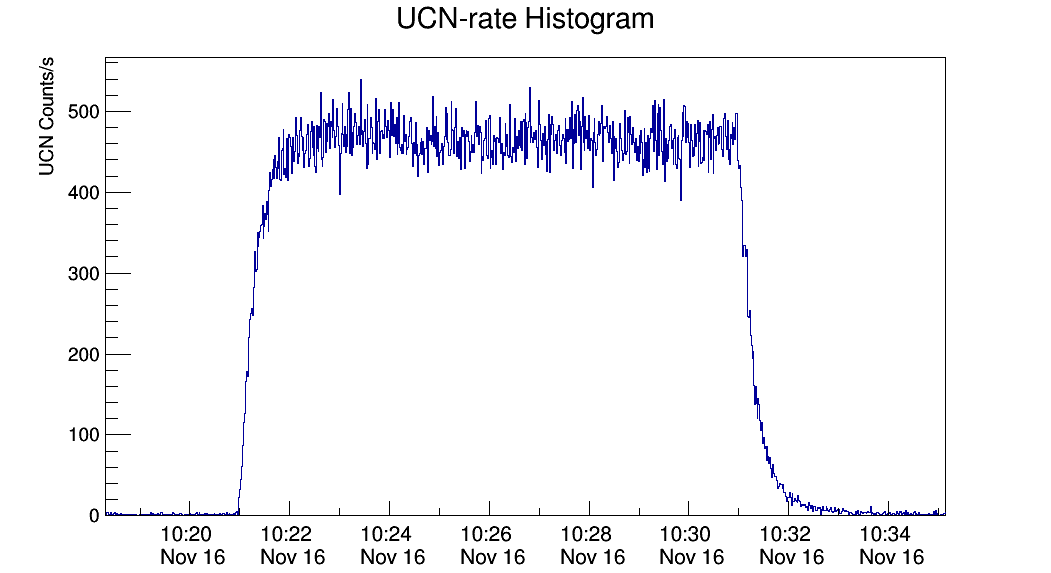
\includegraphics[width=0.9\textwidth]{steadystate_point3muA.png}
  \caption{UCN rate at the steady-state production mode with 0.3~$\mu$A proton beam
    current. The UCN rate reaches a constant value of 450 UCN counts/s.}
  \label{fig:UCNRate_steadystate}
\end{figure}

At lower beam currents such as 0.3~$\mu$A the UCN rate remains
constant throughout the whole target irradiation time as shown in
Fig.~\ref{fig:UCNRate_steadystate}. An example of a steady-state UCN
production at 3~$\mu$A is shown in
Fig.~\ref{fig:UCNRate_steadystate_highbeam}. Since the proton beam
current is high, the UCN rate does not remain a constant. Here the
maximum UCN rate is observed near the start of the target
irradiation. As the target irradiation continues, the heat load on the
cryostat increases the temperature and the upscattering rate in the
superfluid helium. As a result, the UCN rate decreases. The change in
the temperature is shown in Fig.~\ref{fig:UCNRate_temp}. Throughout
the target irradiation time the temperature of the superfluid helium
increases and once the irradiation stops the temperature starts to go
down.


\begin{figure}[h!]
  \centering
  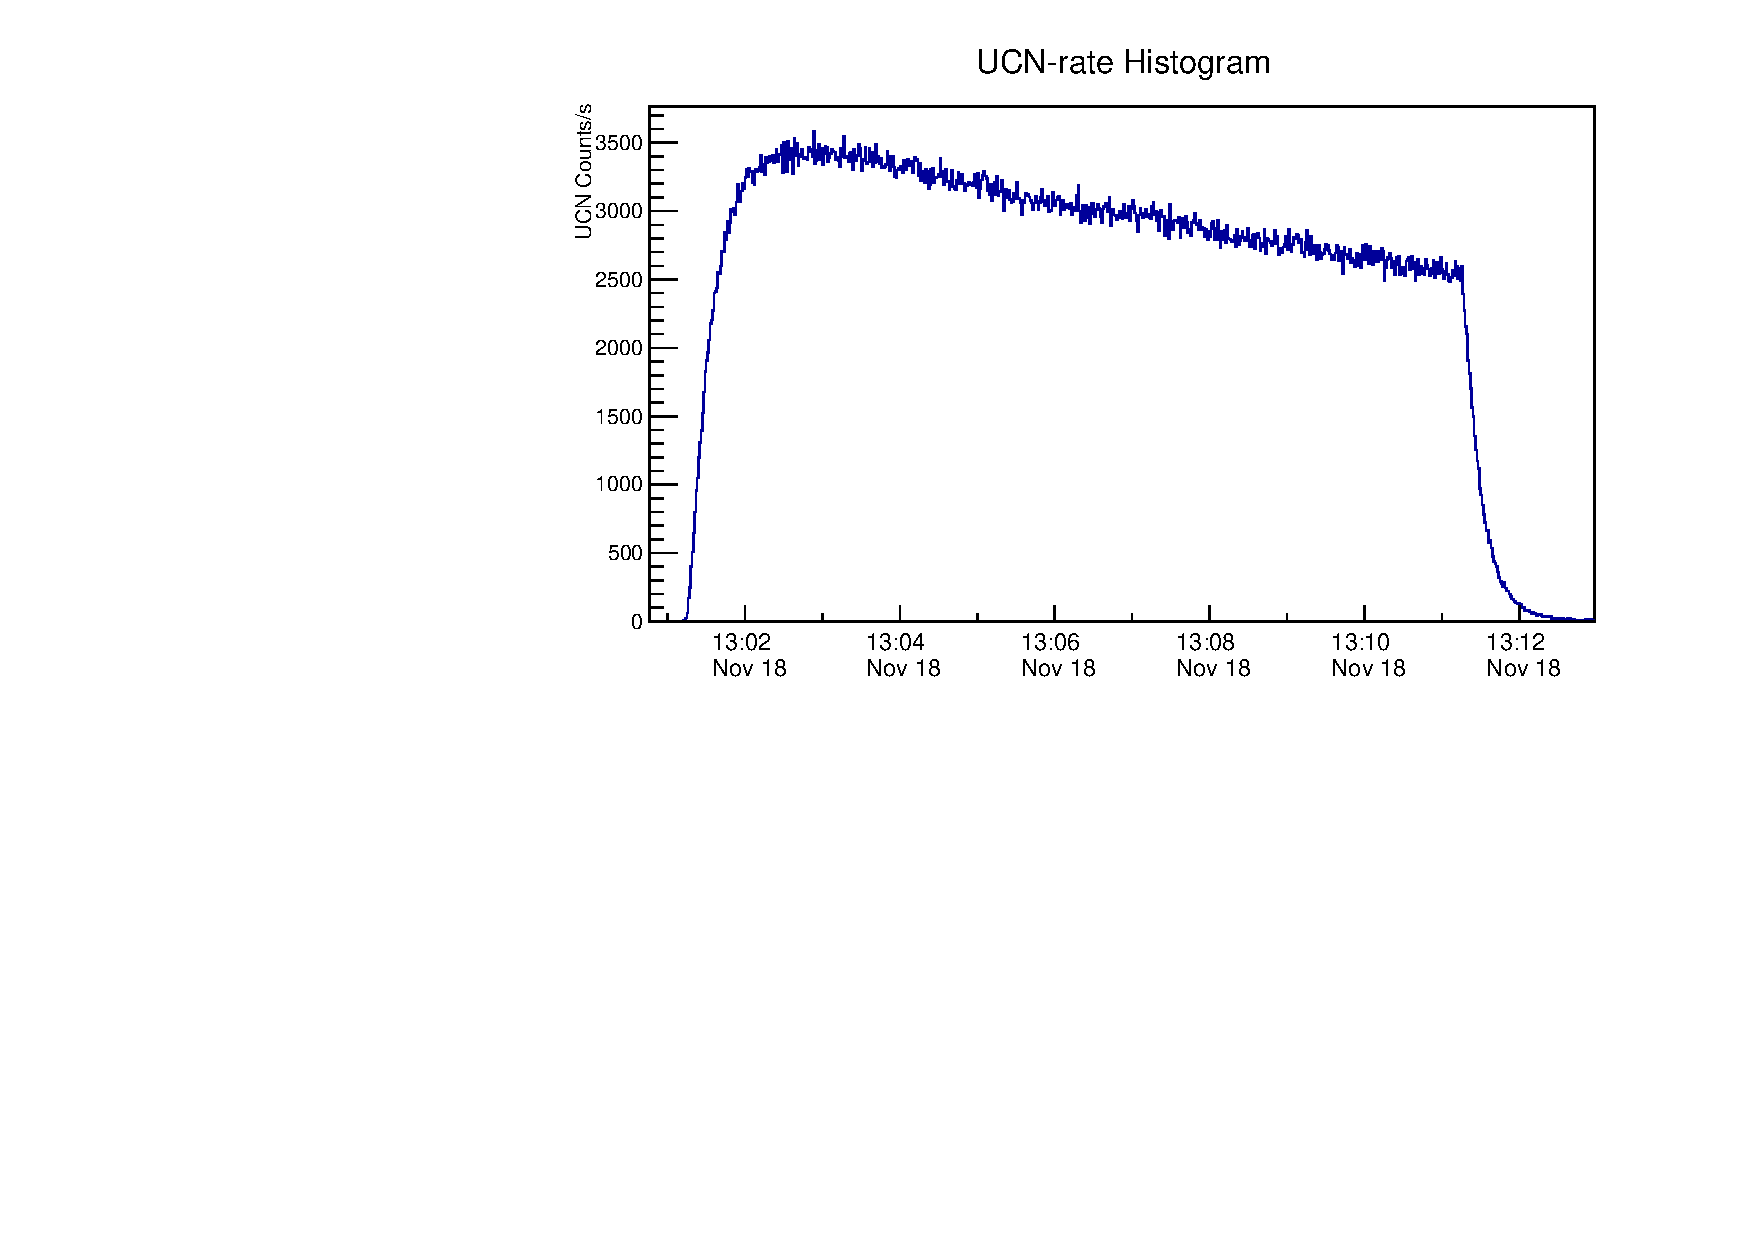
\includegraphics[width=0.9\textwidth]{654_UCNRate.pdf}
  \caption{The UCN rate at 3~$\mu$A beam current at 10~min irradiation
    time at the steady-state mode of operation. The UCN valve is left
    open throughout the measurement cycle. Quickly after the start of
    the target irradiation the UCN rate in the detector goes up. The
    target irradiation creates heatload on the cryostat and superfluid
    helium which gives rise to a slow temperature increase in the
    source. As a result, the UCN rate goes down due to the higher
    upscattering rate.  }
  \label{fig:UCNRate_steadystate_highbeam}
\end{figure}

\begin{figure}[h!]
  \centering
  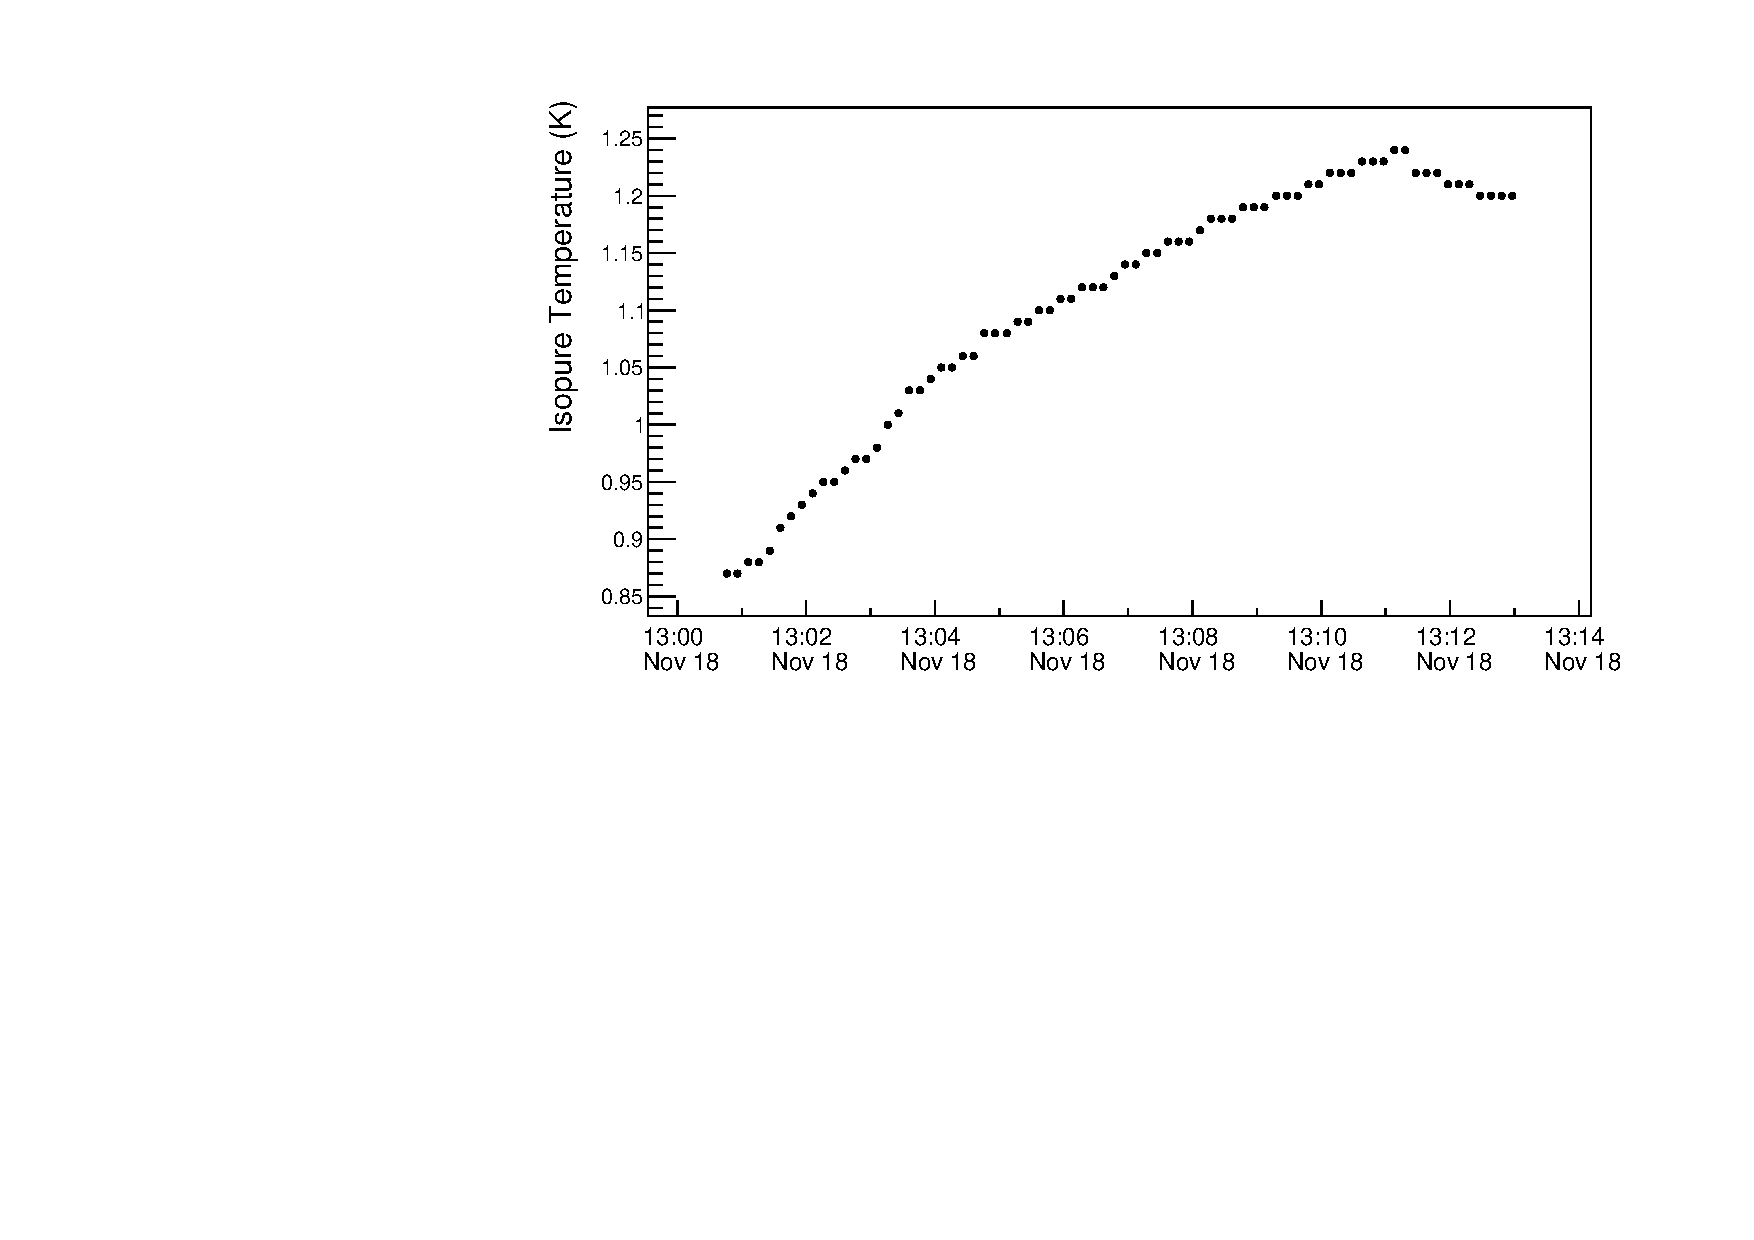
\includegraphics[width=0.9\textwidth]{UCNRate_temp.pdf}
  \caption{ The temperature of the superfluid helium~(TS12) for the
    steady state mode of operation at 3~$\mu$A beam current and 10~min
    target irradiation. After the irradiation stops, the temperature
    starts to go down. }
  \label{fig:UCNRate_temp}
\end{figure}


The steady-state UCN rate measurements were conducted at different
proton beam currents leading to different temperature changes for all
temperature sensors. The result of all those measurements and
comparison to simulations are discussed in Section~\ref{sec:pentrack}.


%are shown in
%Fig.~\ref{fig:rate_vs_temp}. Here the vertical axis is the measured
%UCN rate normalized to the proton beam current and the horizontal axis
%is the temperature of the superfluid helium for all temperature
%sensors.


%\begin{figure}[h!]
%  \centering
%  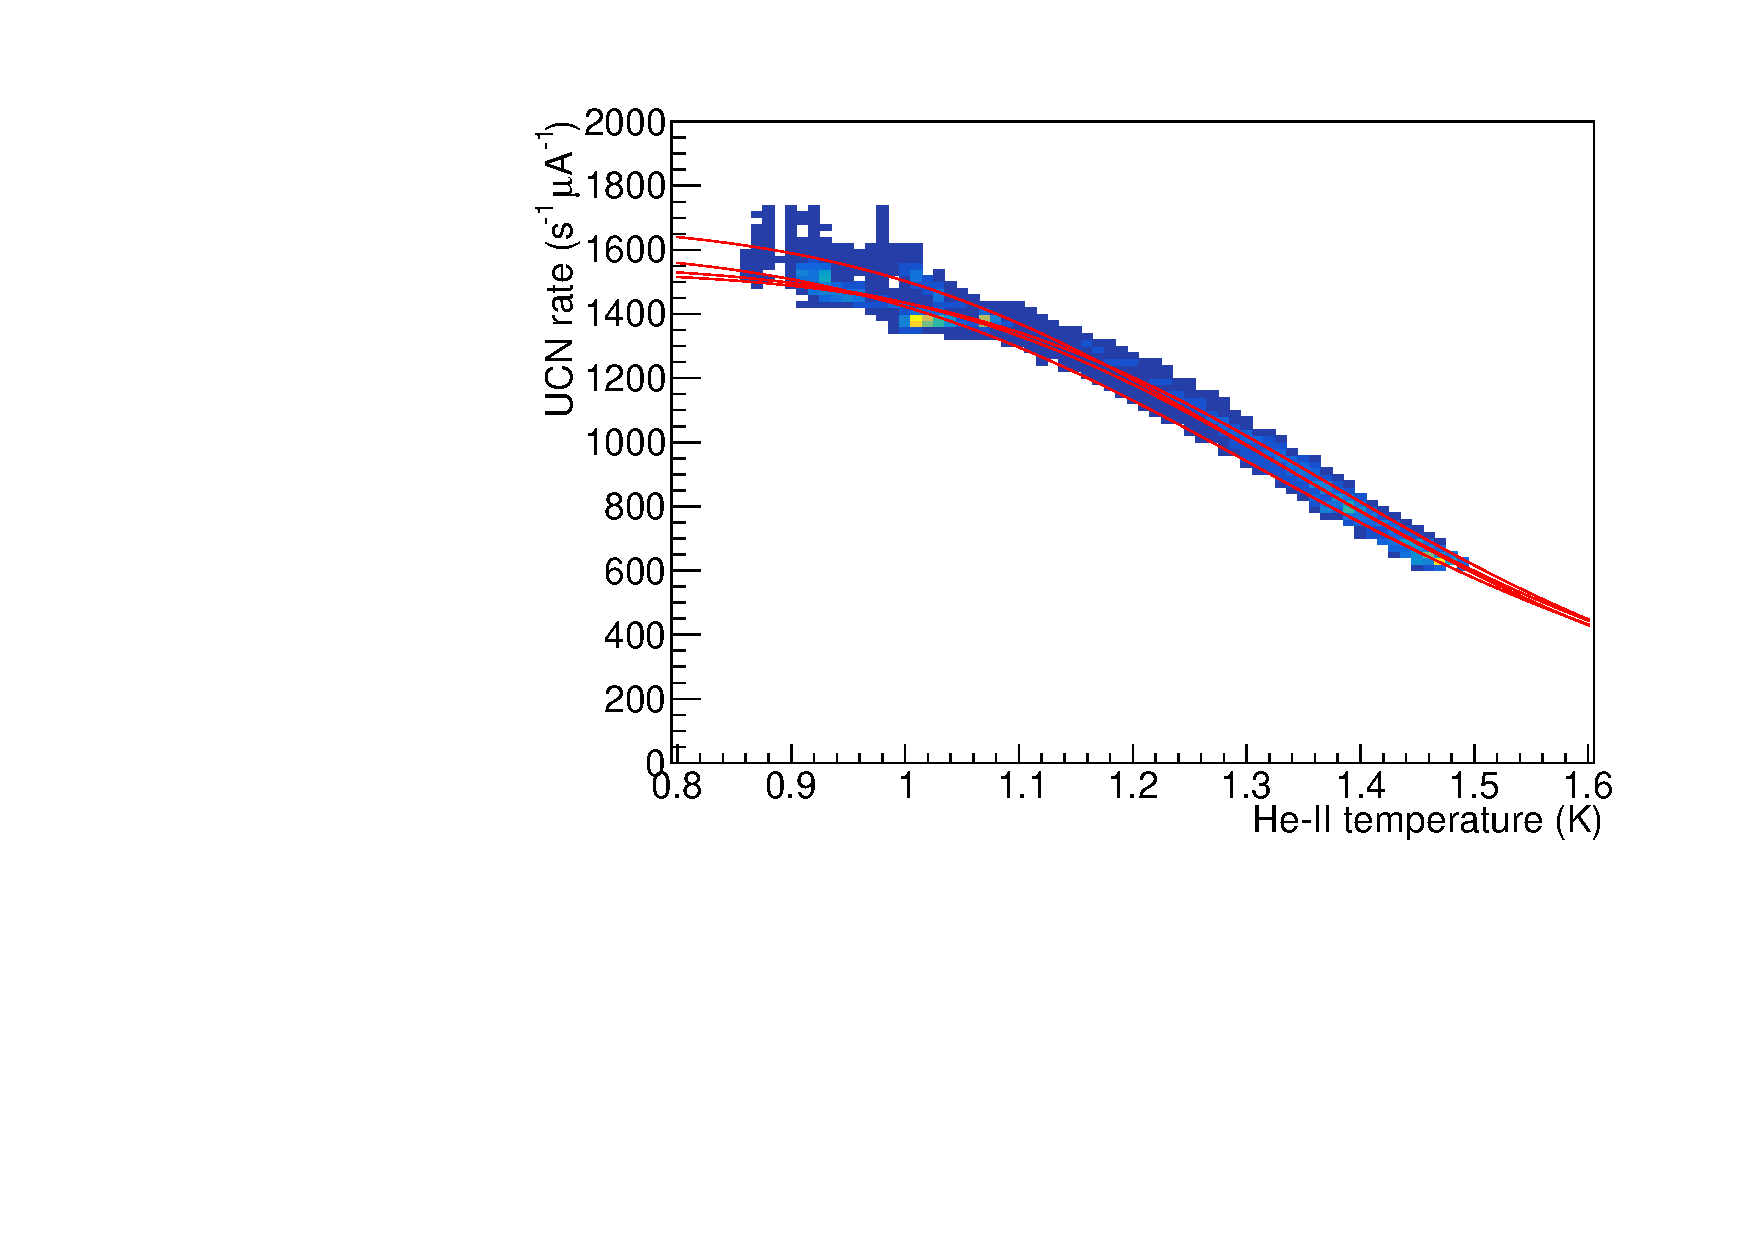
\includegraphics[width=0.7\textwidth]{rate_vs_temp.pdf}
%  \caption{Histogram of measured UCN rates and temperatures from all
%    four temperature sensors while the target is continuously
%    irradiated with the UCN valve open. The four solid lines are fits
%    of equation~\ref{eq:steadystaterate} to the data for each individual temperature
%    sensor.}
%  \label{fig:rate_vs_temp}
%\end{figure}


%The rate of the detected UCN is given by

%\begin{equation}
%  \label{eqn:rate}
%  R = \frac{P \tau_3}{\tau_d} = \frac{P \tau_d^{-1}}{\tau_\mathrm{wall,2}^{-1} + \tau_d^{-1} + f_\mathrm{He,3}\tau_\mathrm{He}^{-1}}
%\end{equation}
%where $\tau_d^{-1}$ is the loss rate in the detector,
%${\tau_\mathrm{wall,2}}^{-1}$ is the UCN guide wall loss and
%$\tau_\mathrm{He}^{-1}$ is the loss rate in the superfluid helium.
%Assuming $\tau_\mathrm{He}^{-1} = B \left( T \right)^a$ the
%Eqn.~\ref{eqn:rate} could be written as

%\begin{equation}
%R(T) = \frac{c}{1 + b \left( \frac{T}{\SI{1}{\kelvin}} \right)^{a}}
%\label{eq:steadystaterate}
%\end{equation}
%where \large
%$b = \frac{f_{\mathrm{He,3}}B}{\tau^{-1}_{\mathrm{wall,2}}
%  +\tau^{-1}_d}$ \normalsize and \large
%$c = \frac{P\tau^{-1}_d}{\tau^{-1}_{\mathrm{wall,2}} +\tau^{-1}_d}$
%\normalsize.  Eqn.~\ref{eq:steadystaterate} can be used to fit the
%data shown in Fig.~\ref{fig:rate_vs_temp}.  Since the four temperature
%sensors in the superfluid helium deviate by up to \SI{0.1}{\kelvin},
%the rate for each temperature sensor is fitted individually (see
%table~\ref{tab:steadystateparams}). The exponent $a$ can be directly
%determined this way, giving
%\begin{equation}
%a = 7.02 \pm 0.02_\mathrm{stat.} \pm 0.53_\mathrm{syst.},
%\label{eq:a}
%\end{equation}
%which is in good agreement with the theoretical prediction of $a = 7$
%(see Sec.\ref{sec:upscattering}). Here the statistical error comes
%from the fit and the systematic error comes from the temperature
%difference from the sensors and their propagated error.


%The other parameters are
%\begin{align}
%\label{eq:b}
%  b =&  0.0995 \pm 0.0007_\mathrm{stat.} \pm 0.0298_\mathrm{syst.} \\
%  c =& (1610 \pm 1_\mathrm{stat.} \pm 75_\mathrm{syst.}) \, \si{\per\second}
%\end{align}

%\begin{table}[h!]
%  \centering
%  \begin{tabular}{|c|c|c|c|}
%    \hline
%      Temp. sensor & $a$ & $b$ & $c$ (\si{\per\second}) \\
%      \hline
%      TS11 & $7.55 \pm 0.03$ & $0.0697 \pm 0.0009$ & $1535 \pm 1$ \\
%      \hline
%      TS12 & $6.48 \pm 0.03$ & $0.1293 \pm 0.0016$ & $1606 \pm 2$ \\
%      \hline
%      TS14 & $7.34 \pm 0.03$ & $0.0832 \pm 0.0011$ & $1555 \pm 2$ \\
%      \hline
%      TS16 & $6.67 \pm 0.04$ & $0.1215 \pm 0.0019$ & $1685 \pm 3$ \\
%      \hline
%    \end{tabular}
%  \caption{Parameters determined by fitting equation
%    \ref{eq:steadystaterate} to the measured rates shown in
%    fig. \ref{fig:rate_vs_temp} for each individual temperature
%    sensor.}
%  \label{tab:steadystateparams}
%\end{table}



\subsection{UCN Yield Over the Experiment Period}

The total UCN counts for our standard measurements at 1~$\mu$A beam
current and 60~s irradiation time over the course of the experimental
run is shown in Fig.~\ref{fig:UCNCounts_time}. The graph shows an
overall decrease of about $\sim$~40\% over the course of the
experimental run.  The source volume is connected to a long UCN guide
sealed with an O-ring. It is expected that the rest gas to contaminate
the source every time the UCN valve is opened. This caused a reduction
in the UCN yield~(and storage lifetime as shown later in
Section~\ref{sec:storage_overall}) over the course of the
measurement. In addition, the changes in the UCN guide geometry in the
latter half of the run pottentially affected this drop.


\begin{figure}[h]
  \centering
  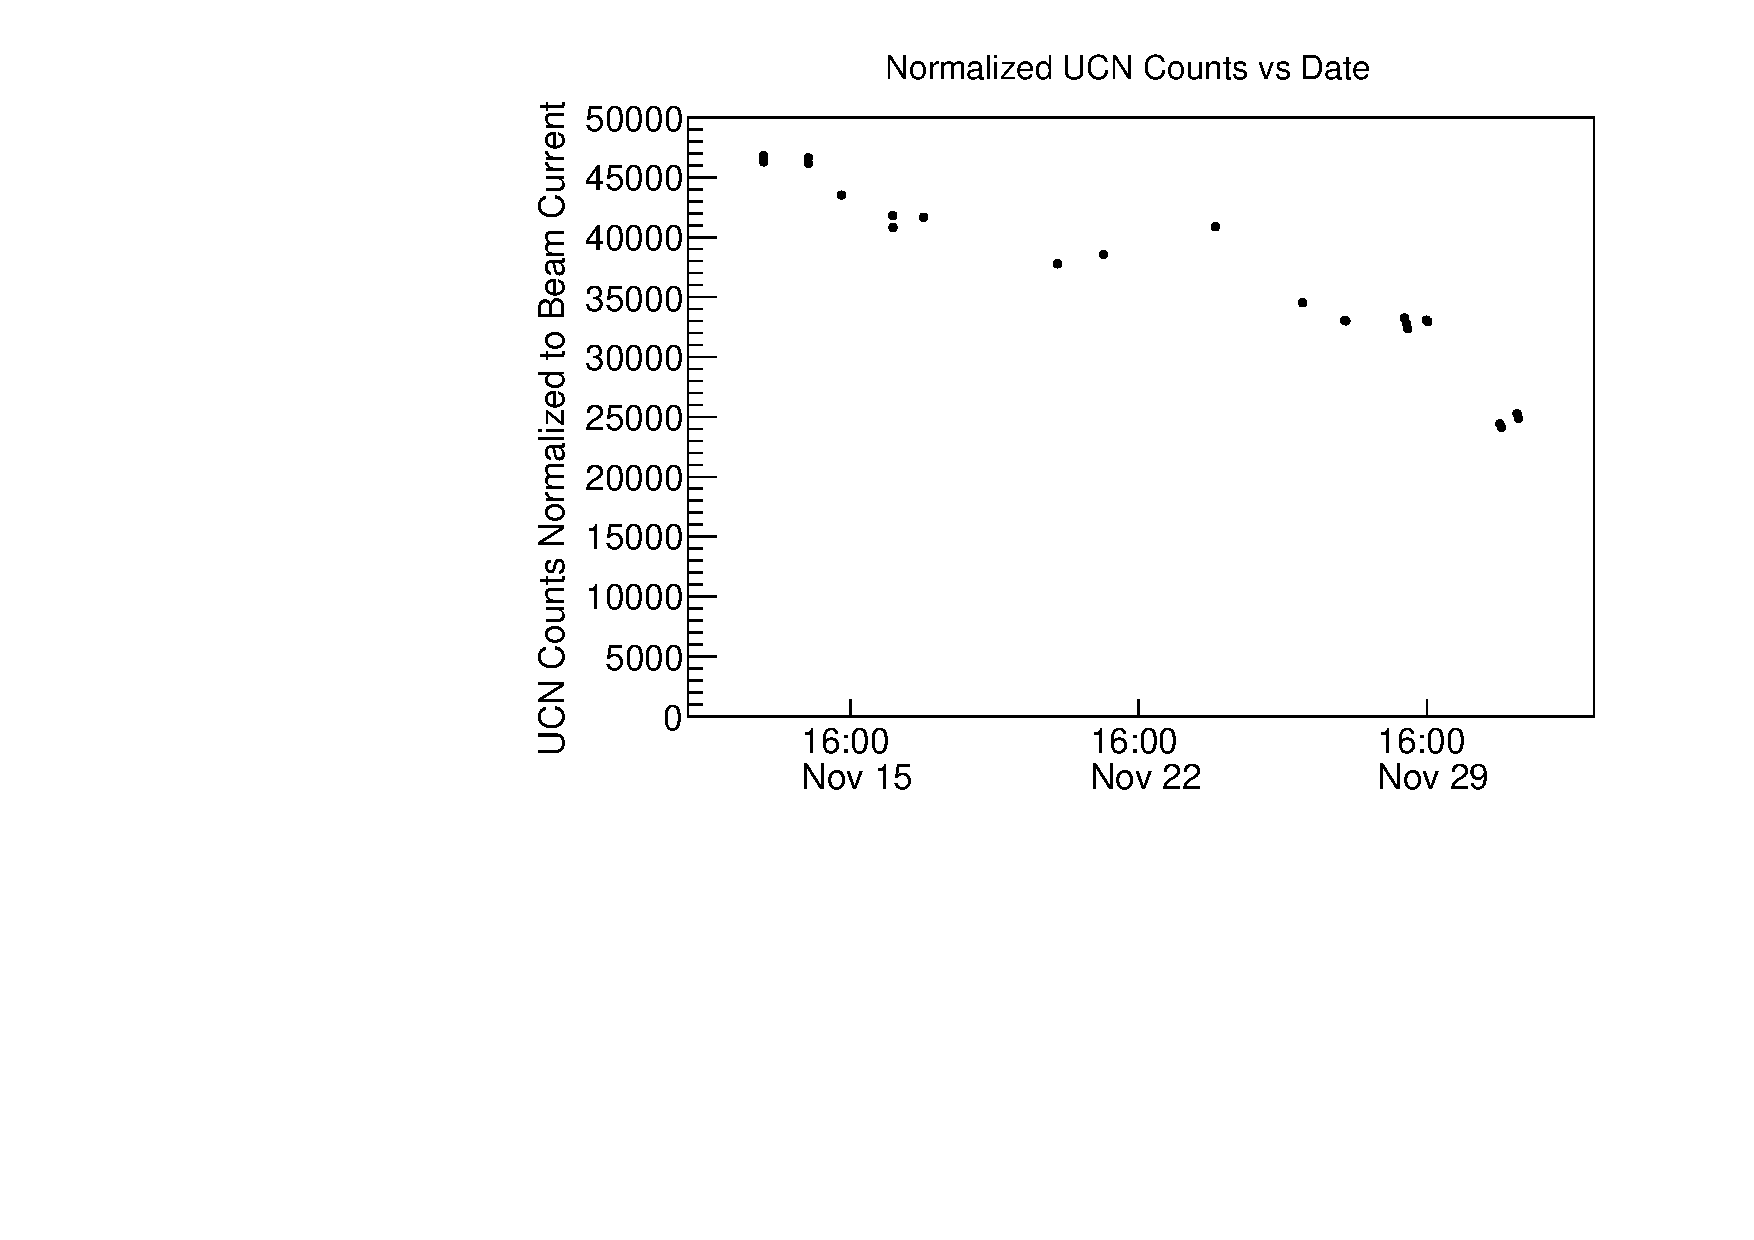
\includegraphics[width=0.9\textwidth]{UCNCounts_vs_time.pdf}
  \caption{The total UCN counts extracted from the source for 1~$\mu$A
    beam current and 60~s irradiation time at different days during
    the experimental run. }
  \label{fig:UCNCounts_time}
\end{figure}

\section{UCN Storage Lifetime~\label{storagelifetime}}

The total number of detected UCN strongly depends on the storage
lifetime of the source $\tau_1$~(See Eqn.~\ref{eqn:tau1}) which
indicates the performance of the UCN source. The storage lifetime of
UCN is determined by measuring the detected UCN at different valve
open delay times right after the irradiation stops.  The typical
chosen values are 0~s, 5~s, 10~s, 20~s, 30~s, 60~s, 80~s, 120~s and
170~s.
% For most of the experiments, the order in which the delay to the
% valve open time was applied was as following: 0~s, 170~s, 20~s,
% 120~s, 50~s, 80~s, 30~s and 5~s.
The exponential decay constant in the fit function to the total UCN
counts without the background for different valve open delay times is
the total storage lifetime in the source.

Fig.~\ref{fig:storage_all} shows several UCN cycles for the standard
1~$\mu$A proton beam current and 60~s target irradiation time. The
difference in the maximum detected UCN rate is due to different valve
open delay times.
\begin{figure}[h!]
  \centering
  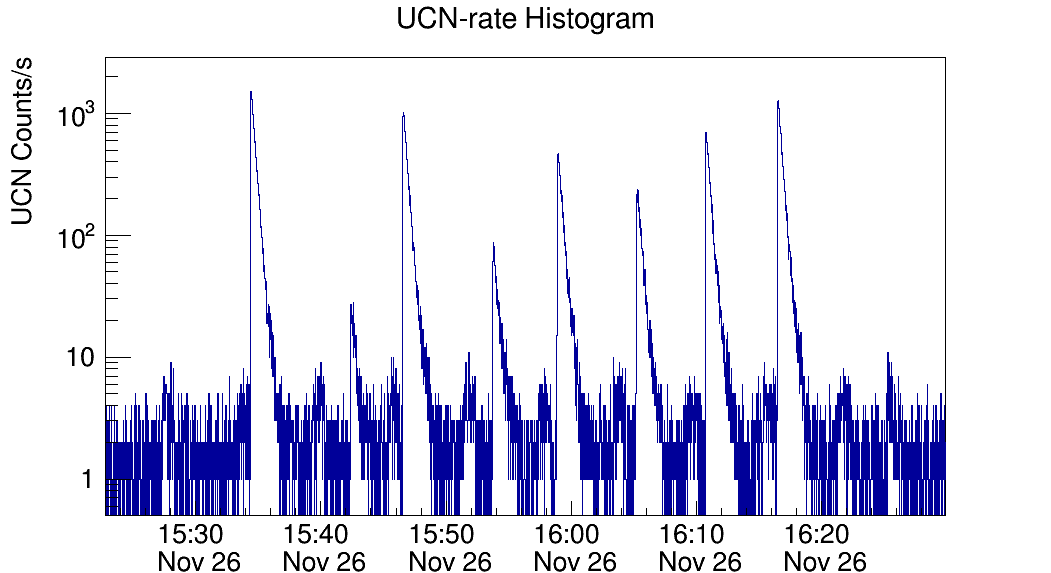
\includegraphics[width=0.9\textwidth]{storagetime_all.png}
  \caption{UCN cycles at different valve open delay time for 1~$\mu$A
    beam current and 60~s target irradiation time.}
  \label{fig:storage_all}
\end{figure}
Fig.~\ref{fig:storage_example} shows the total UCN counts~(background
subtracted) versus the valve open delay time for 1~$\mu$A proton beam
current and 60~s target irradiation time. The longer delay times give rise to
lower UCN counts due to the loss mechanisms. The one exponential fit
function
\begin{equation}
\text{UCN counts} = A e^{-t/\tau_1}
\end{equation}
determines the storage lifetime $\tau_1$. At 170~s valve open delay
time, the total UCN counts are not consistent with what the fit
function predicts due to low statistics. However, the result of the
fit is not driven by this inconsistency as it has a negligible effect
on the extrected storage lifetime.

\begin{figure}[h!]
  \centering
  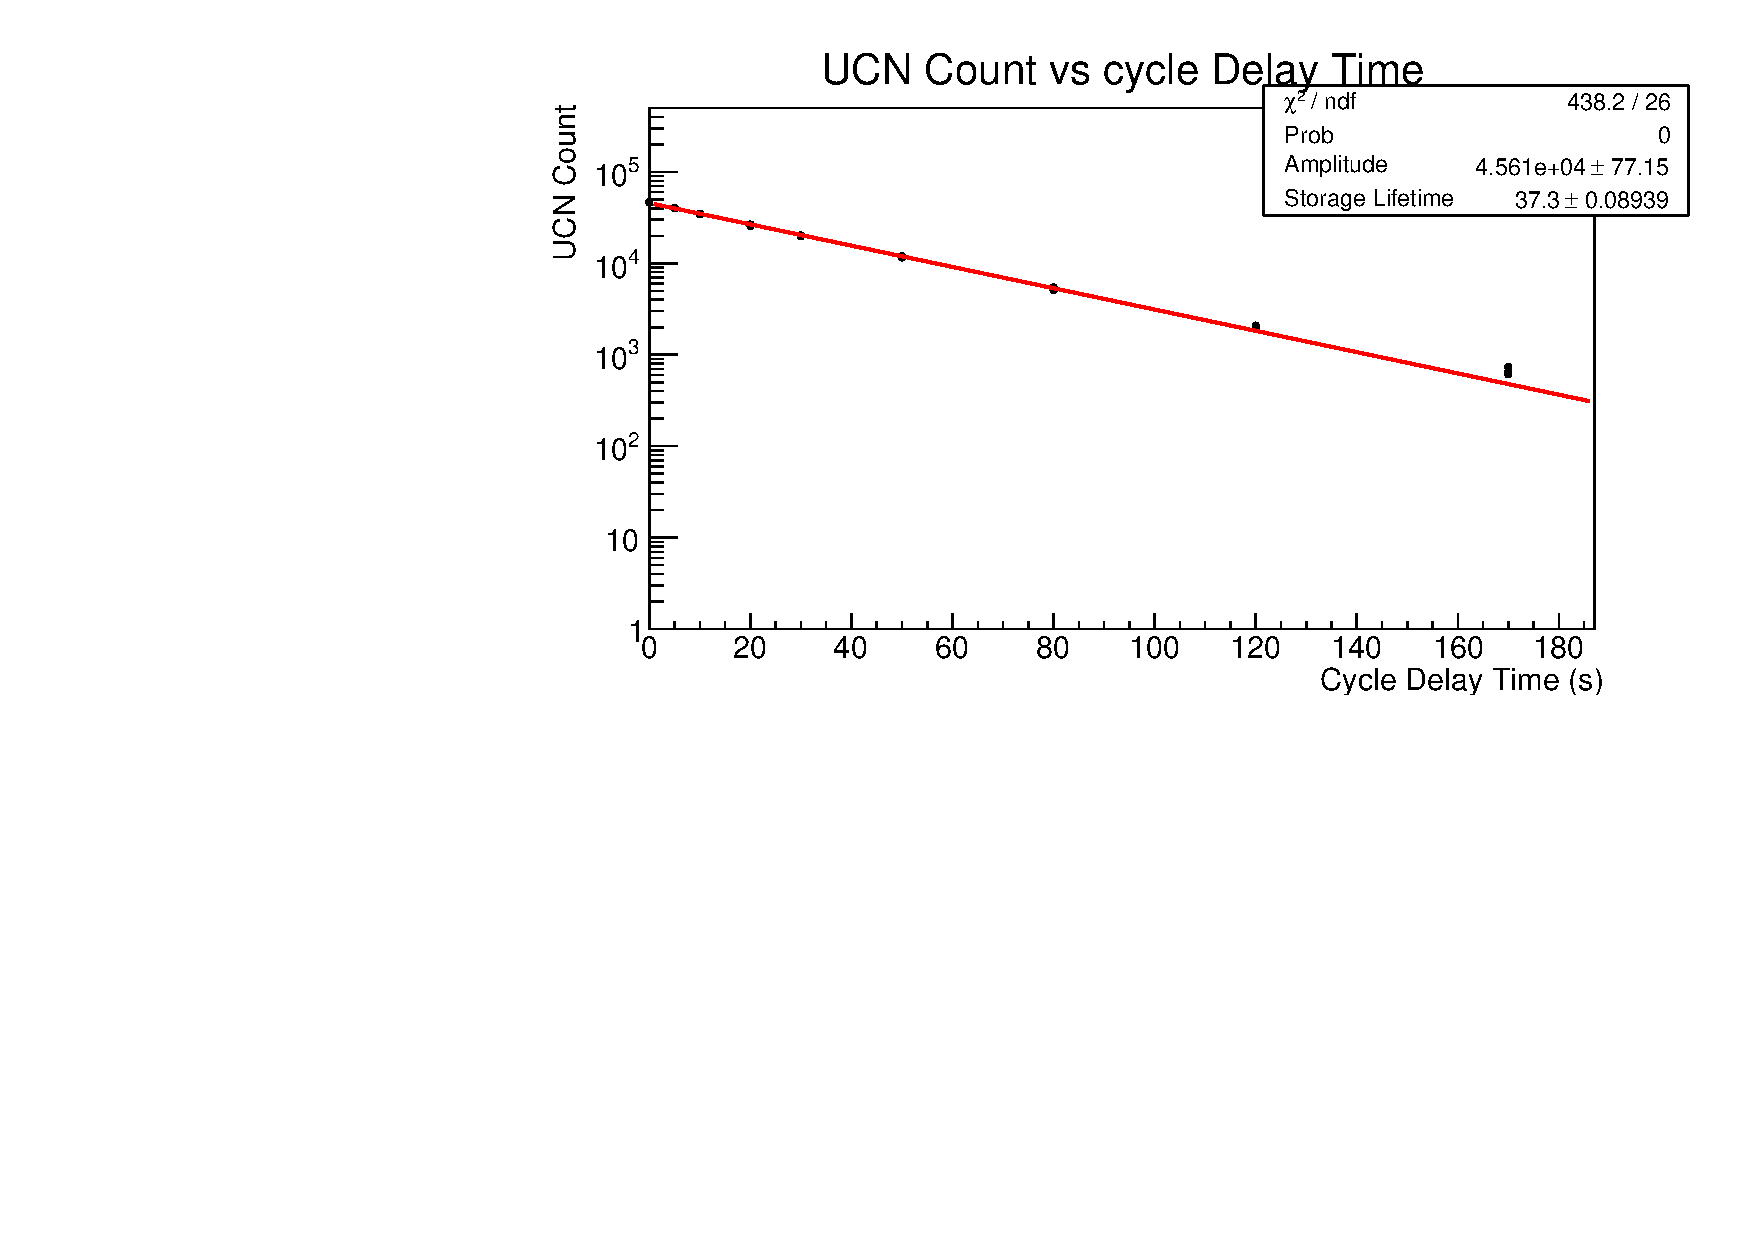
\includegraphics[width=0.9\textwidth]{17002_StorageLifetime.pdf}
  \caption{The total UCN counts at different valve open delay times
    for 1~$\mu$A beam current and 60~s irradiation time. The red line
    is the one exponential fit. }
  \label{fig:storage_example}
\end{figure}

Below the result of the storage lifetime measurements are presented.

\subsection{Storage Lifetime Versus Beam Current and Irradiation Time}
The storage lifetime of the UCN source is measured at different proton
beam currents and different target irradiation times for better
optimization of the source. The result of those measurements is shown
in Fig.~\ref{fig:storage_beam_irrad}. Here the vertical axis shows the
storage lifetime in the source in seconds and the horizontal axis
shows the proton beam current in $\mu$A. Each marker represents a
target irradiation time. At lower beam currents, the duration of the
target irradiation does not make a significant difference in the
storage lifetime. At higher proton beam currents, the longer the
irradiation time, the lower the storage lifeimte.

In summary, irradiating the target at high proton beam currents for
longer irradiation times creates a higher heat load on the UCN source
which leads to higher upscattering rates and as a result lower UCN
storage lifetime in the source.

\begin{figure}[h!]
  \centering
  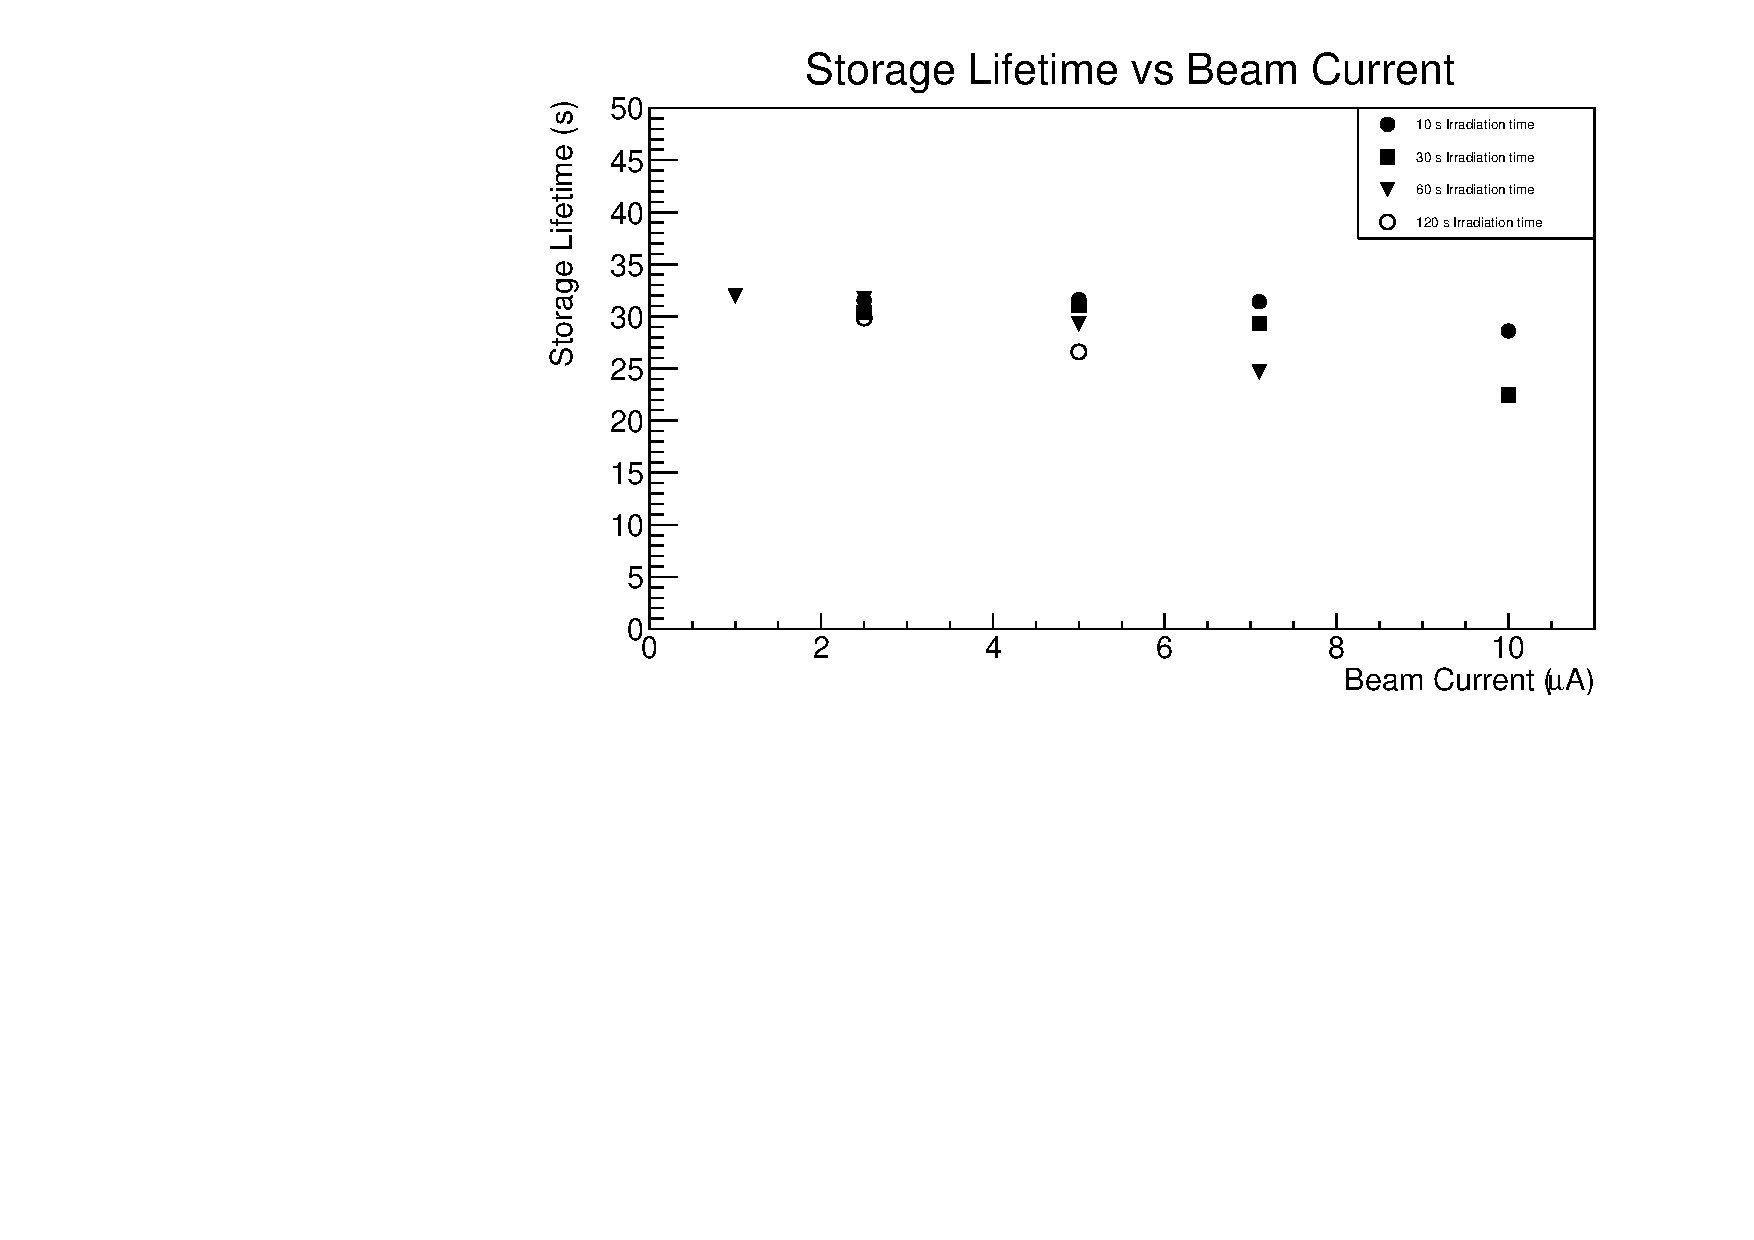
\includegraphics[width=0.9\textwidth]{StorageLifetime_17009_and_17009A.pdf}
  \caption{Storage lifetime in the source at different irradiation
    times and proton beam currents. Different markers refer to
    different target irradiation times. At longer irradiation times
    and higher beam currents the storge lifetime decreases due to the
    increased heat load in the source and an increase in the
    superfluid helium temperature. }
  \label{fig:storage_beam_irrad}
\end{figure}


\subsection{Storage Lifetime Versus Isopure Helium Temperature}
The storage lifetime of UCN was also measured at different
temperatures of the superfluid helium. In this experiment, the
temperature of superfluid was increased by using the heater tapes
wrapped around the UCN bottle. The heater powers were set to increase
the temperatures by a certain amount. Once the temperatures reached a
stable state, the target irradiation started.

The result of this measurement is shown in
Fig.~\ref{fig:storagelifetime_vs_temp}. The vertical axis is the
storage lifetime of UCN in seconds and the horizontal axis is the
temperature of the superfluid helium. As mentioned earlier, the four
temperature sensors that measure the temperature of the superfluid
show some discrepancy. As a result, for a given value of the storage
lifetime there are four different values for the temperature of the
superfluid. The horizontal error bars are set as
($T_{\mathrm{max}} - T_{\mathrm{min}}$)/2 as discussed earlier. The
data shows a downward trend. As the temperature of the superfluid
helium increases, the storage lifetime in the source decreases. This
is due to the higher upscattering rate in the superfluid helium at
higher temperatures.


%TCN17014
\begin{figure}[h!]
  \centering
  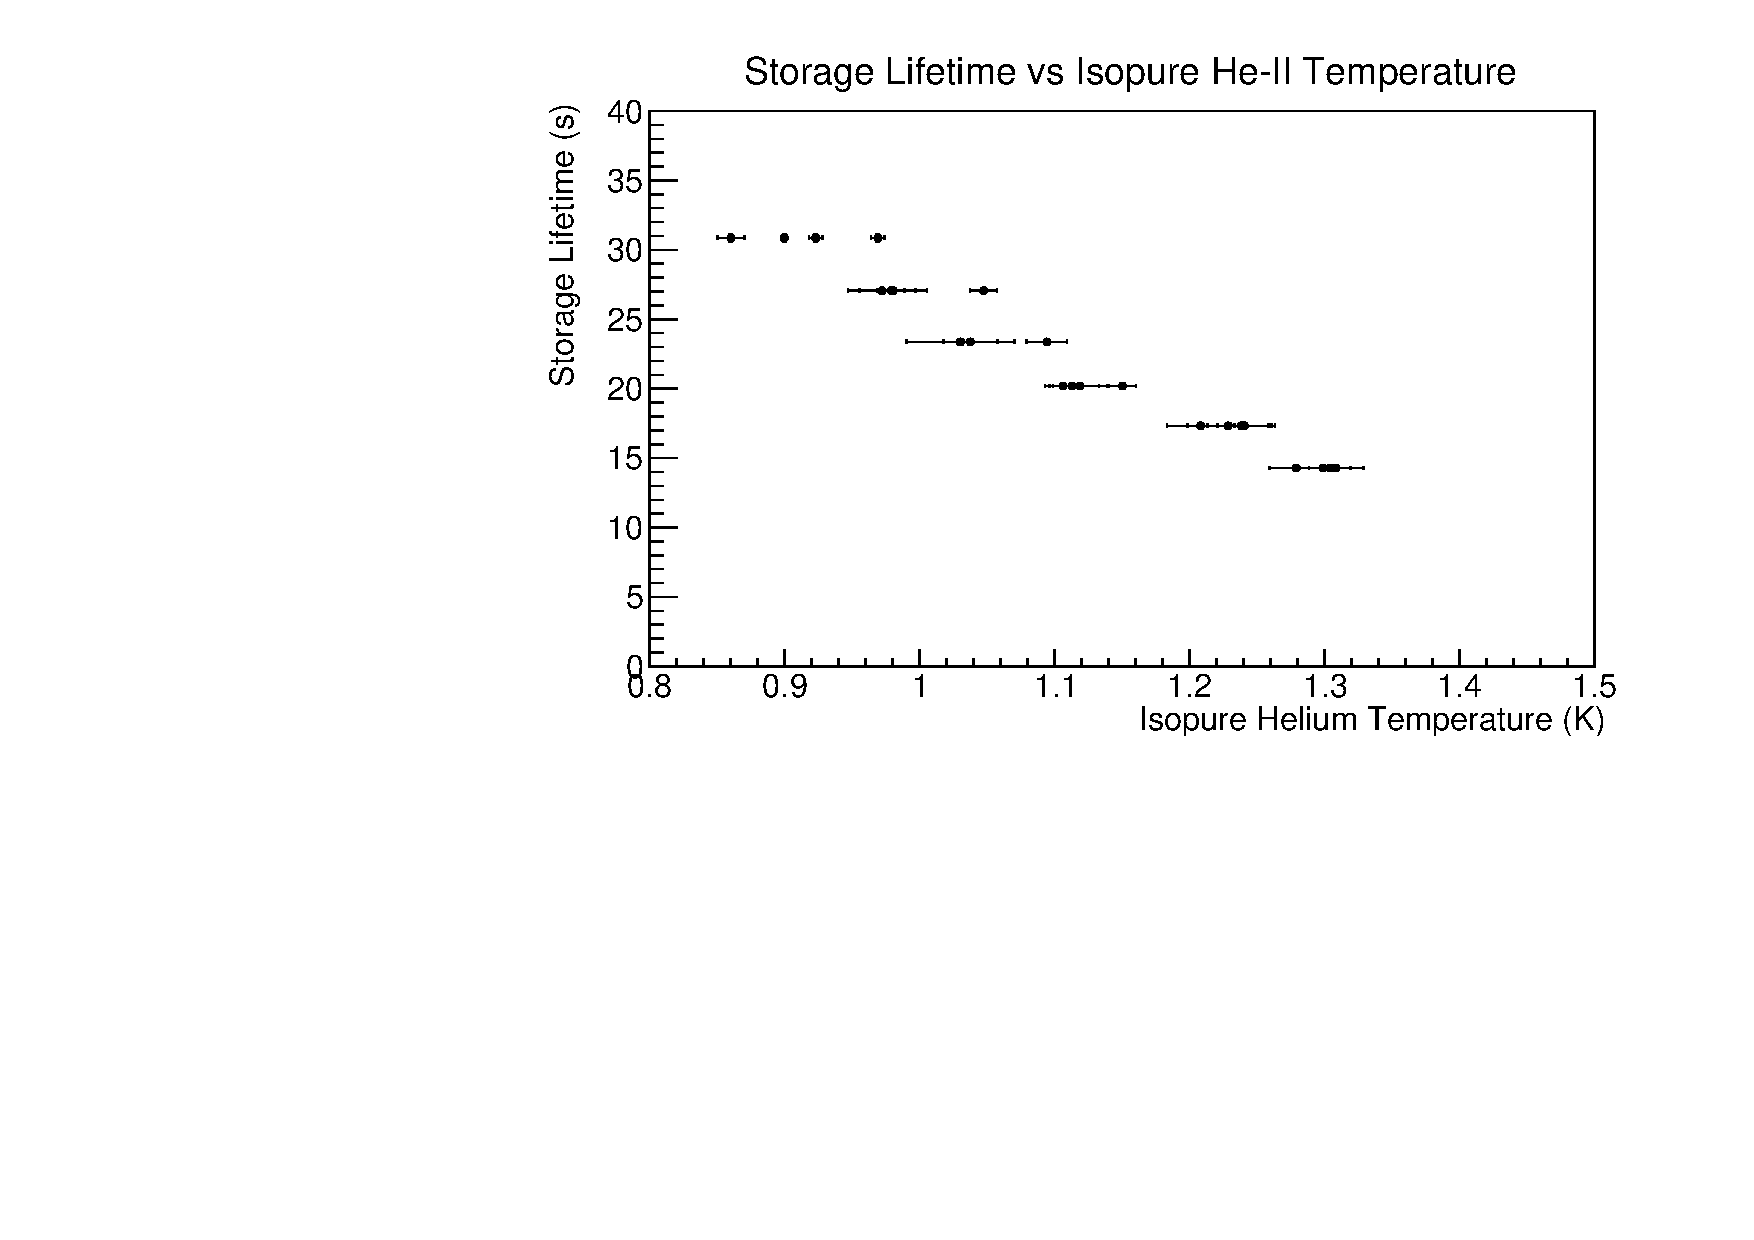
\includegraphics[width=0.9\textwidth]{StorageLifetime_vs_temp.pdf}
  \caption{Storage lifetime of UCN at different isopure helium
    temperatures. In this experiment the temperature of superfluid
    helium was set using heater tapes around the UCN bottle. The
    vertical axis shows the storage lifetime in seconds and the
    horizontal axis shows the superfluid helium temperature in
    Kelvin. As the temperature increases, the storage lifetime
    decreases. This is due to the higher upscattering rate in the
    superfluid helium at higher temperatures.}
  \label{fig:storagelifetime_vs_temp}
\end{figure}


%%%%%%%%%%%%%%
\subsection{Storage Lifetime Over Experimental Period\label{sec:storage_overall}}

The standard storage lifetime measurements were performed on a daily
basis over the course of the experimental run. This includes the
irradiation of the target at 1~$\mu$A proton beam current for 60~s
irradiation time. The result of those measurements are shown in
Fig.~\ref{fig:storagelifetime_overall}. Over a two week period, the
storage lifetime decreased from 37~s to 27~s. This is possibly due to
the contamination in the UCN source after opening the UCN valve.


\begin{figure}[h!]
  \centering
  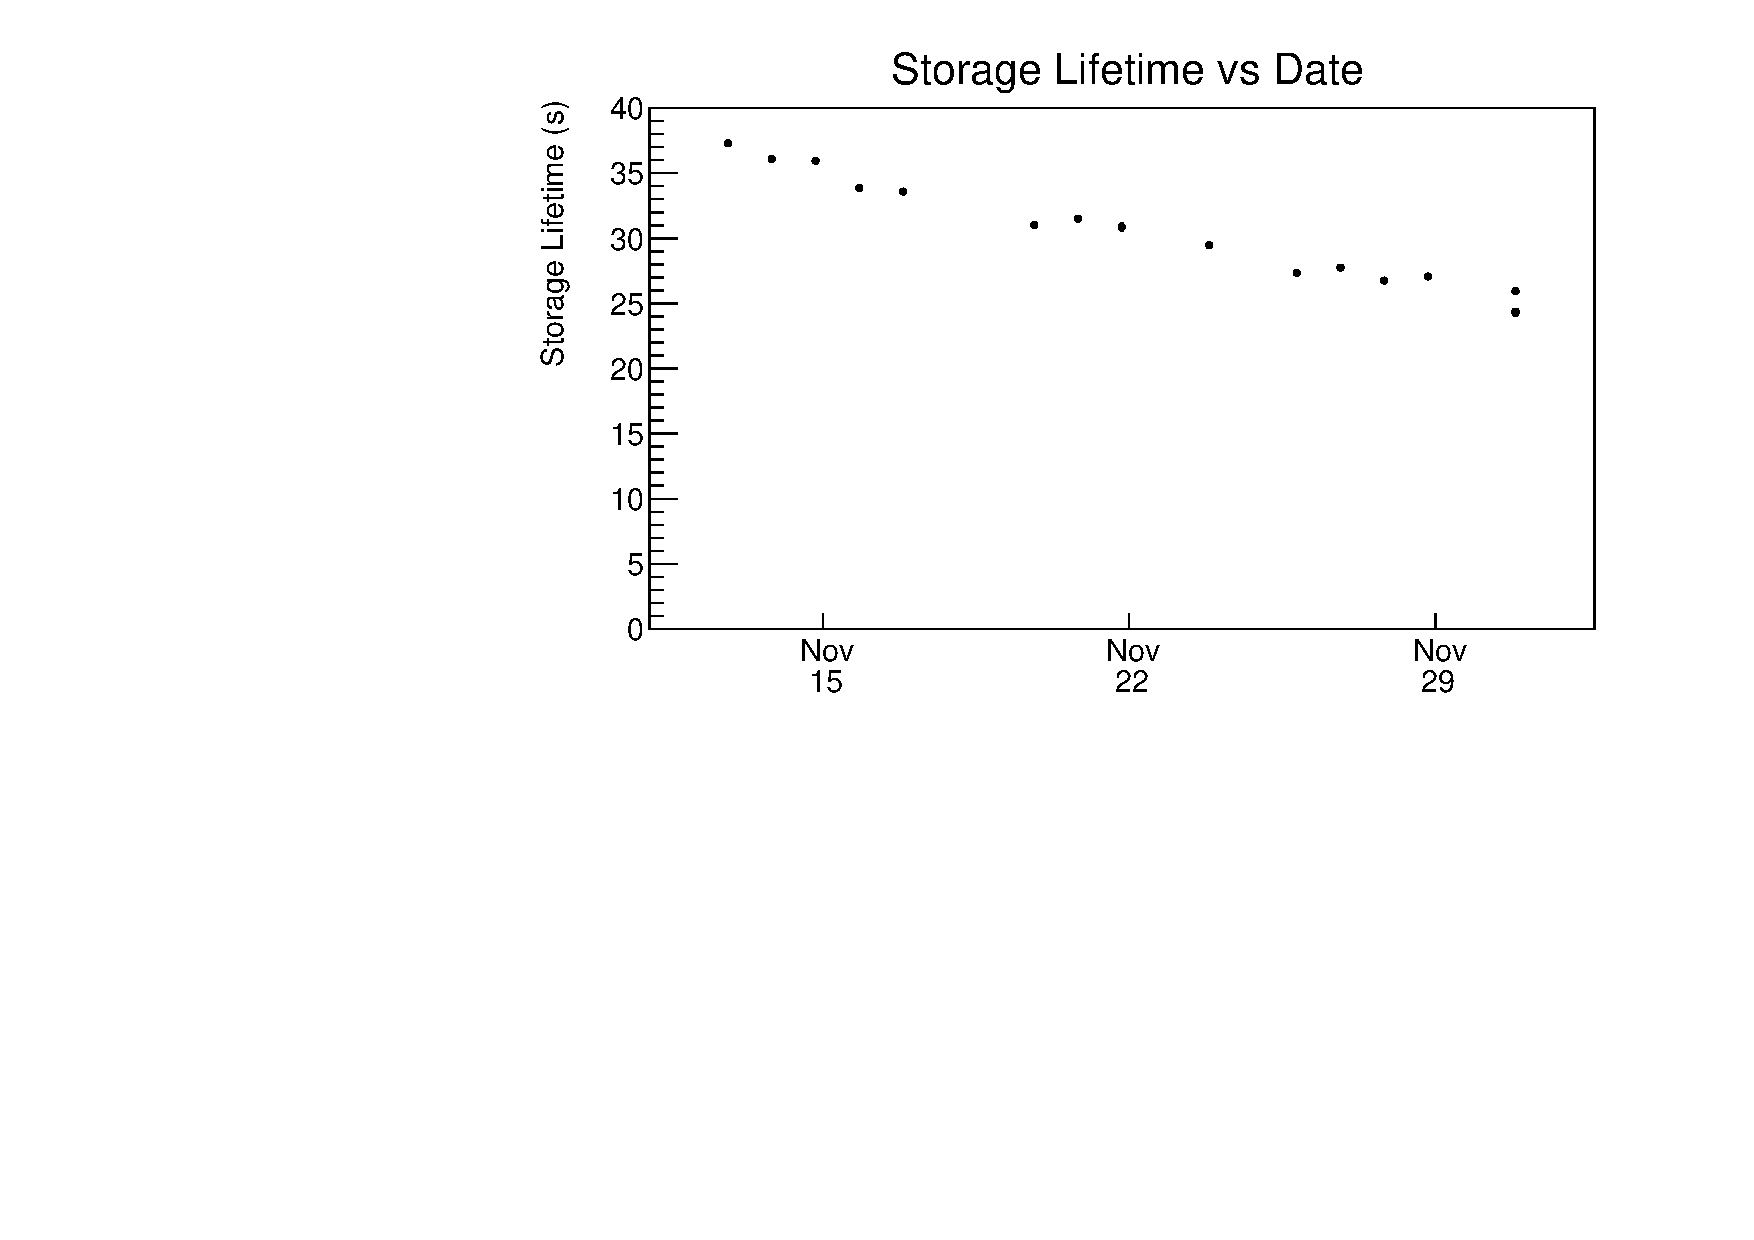
\includegraphics[width=0.9\textwidth]{storageLifetime_vs_time.pdf}
  \caption{Storage lifetime of the source over the experimental run. A
    2\% daily decrease in the storage lifetime is observed possibly
    due to the contamination in the source after opening the UCN
    valve.}
  \label{fig:storagelifetime_overall}
\end{figure}



\section{PENTrack Simulations\label{sec:pentrack}}

For better understanding of the loss mechanisms of UCN, the
experiments were also simulated in
PENTrack~\cite{schreyer2017pentrack}. PENTrack is a particle tracking
simulation software which simulates the trajectories of UCN and their
decay products~({\it{e.g.}} Protons and Electrons) and their spin
precession in complex geometries in Electric and Magnetic fields by
solving the relativistic equation of motion.

To simulate the UCN storage and transport, an exact model of the UCN
guides for PENTrack was build by the TUCAN team including the burst
disk, the actual shape of the UCN valve in open and closed state,
pinhole, foil and detector. Here the result of such simulations are
presented.
%%%%%%%%%%%%%%%%%%%%%%%%%%%%%%%%%%%%%%%%%%%%%%%%%%
\subsection{UCN Guide Diffusivity\label{sec:diffusivity}}
As discussed in Chapter~\ref{chap:intro}, UCN interacts with all four
fundamental forces. To describe the interaction of UCN with matter, a
complex optical potential is used to describe matters:
\begin{equation}
  \label{eqn:fermipotential}
  U = V - iW
\end{equation}
where the real part, $V$, depends on the number densities and bound
coherent scattering lengthes of each nucleus species. The imaginary
part, $W$, depends on the loss cross-section for a given velocity.
Upon the incidence of the UCN on a surface, it can be scatterd either
specularly or diffusely. The specular reflection by definition is the
reflection of light from a smooth surface at a defined angle and the
diffuse reflection is the reflection by rough surfaces that tend to
reflect light in all directions.

PENTrack simulations were performed to extract the diffusivity of the
UCN guides. PENTrack uses two models to calculate the scattering
distribution of the UCN impinging on the material surface: Lambert
model and the Microroughness~\cite{Steyerl1972}. Experimental
geometries imported in PENTrack are the StL files made through CAD
models. For these simulations, the exact model of the vertical UCN
source was used including the burst disk, the actual shape of the UCN
valve in the open and close state, pinhole foil and the detector.

The abosorption in the foil is set according to the measurements
in~\cite{atchison2009transmission}. The main decetor is modeled with
its two scintillator layes~\cite{jamieson2017characterization} and
their corresponding Fermi potentials and absorption cross-section, as
stated in~\cite{Ban2016}.  In the simulations, it is assumed that the
spectrum of produced UCN is proportional to $\sqrt{E}$. The wall loss
parameters were tuned to give a storge lifetime of
$\tau_1 = 34.9 \pm .8$~s with an upscattering lifetime in the
superfluid of
$\tau_{\mathrm{He}}^{-1} = (390~\mathrm{s})^{-1} =
0.008~\mathrm{s}^{-1}\cdot 0.85^{7}$, resulting in material parameters
shown in Table~\ref{tab:materials}.


\begin{table}
  \centering
\begin{tabular}{|c|c|c|}
  \hline
Material & Fermi pot. (neV) & Diffusivity \\
\hline
He-II ($\tau_\mathrm{He} = \SI{390}{\second}$) & $18.8 - 8.44\cdot10^{-10} i$ & 0.16 \\
Prod. volume (NiP) & $213 - 0.100 i$ & 0.05 \\
Guides (stainl. steel) & $183 - 0.120 i$ & 0.03 \\
%Pinhole (copper) & $171 - 0.0726 i$ & 0.20 \\
Foil (aluminium) & $54.1 - 0.00281 i$ & 0.20 \\
GS30 scintillator & $83.1 - 0.000123 i$ & 0.16 \\
  GS20 scintillator & $103 - 1.24 i$ & 0.16 \\
  \hline
\end{tabular}
\caption{Material parameters used in the PENTrack simulation.~\cite{atchison2009transmission,Ban2016,sears1992neutron}}
\label{tab:materials}
\end{table}

The simulation and the measurement data are both fitted with the fucntion

\begin{equation}
R(t) = R_0 \left[ 1 - \exp \left( -\frac{t - \Delta t}{\tau_\mathrm{rise}} \right) \right] \exp \left( -\frac{t - \Delta t}{\tau_2} \right) + R_B
\end{equation}
After opening the valve at $t=0$. In this equation, $\Delta t$ is the
delay time between opening the valve and detecting the first UCN and
it is 2 to 3~s. The parameter $ R_B$ is the background UCN rate in the
experimental data and is zero in simulations.  The rise time
$\tau_{\mathrm{rise}}$ and fall time~$\tau_2$ are shown in
Fig.~\ref{fig:risefalltime} for a given UCN cycle.  The Lambert model
is used to tune the probablity of UCN being diffusely reflected on the
guide walls to match the rise time and fall
time of the UCN rate in the storage lifetime
measurements~(See Fig.~\ref{fig:falltime} and~\ref{fig:risetime}). The
data is shown by the boxes and the simulation result for different UCN
guide diffusivity is shown by different markers. The experimental data
is best described by the diffusivity of 3~\% and 5~\%.


\begin{figure}[h!]
  \centering
  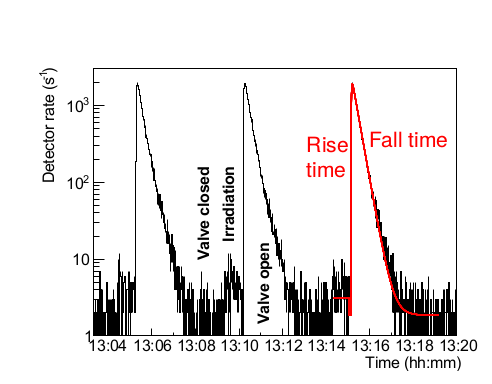
\includegraphics[width=0.8\textwidth]{risefalltime.png}
  \caption{UCN rate with two exponential fit shown in red. The rise
    time and fall time are labled.}
  \label{fig:risefalltime}
\end{figure}



\begin{figure}[h!]
  \centering 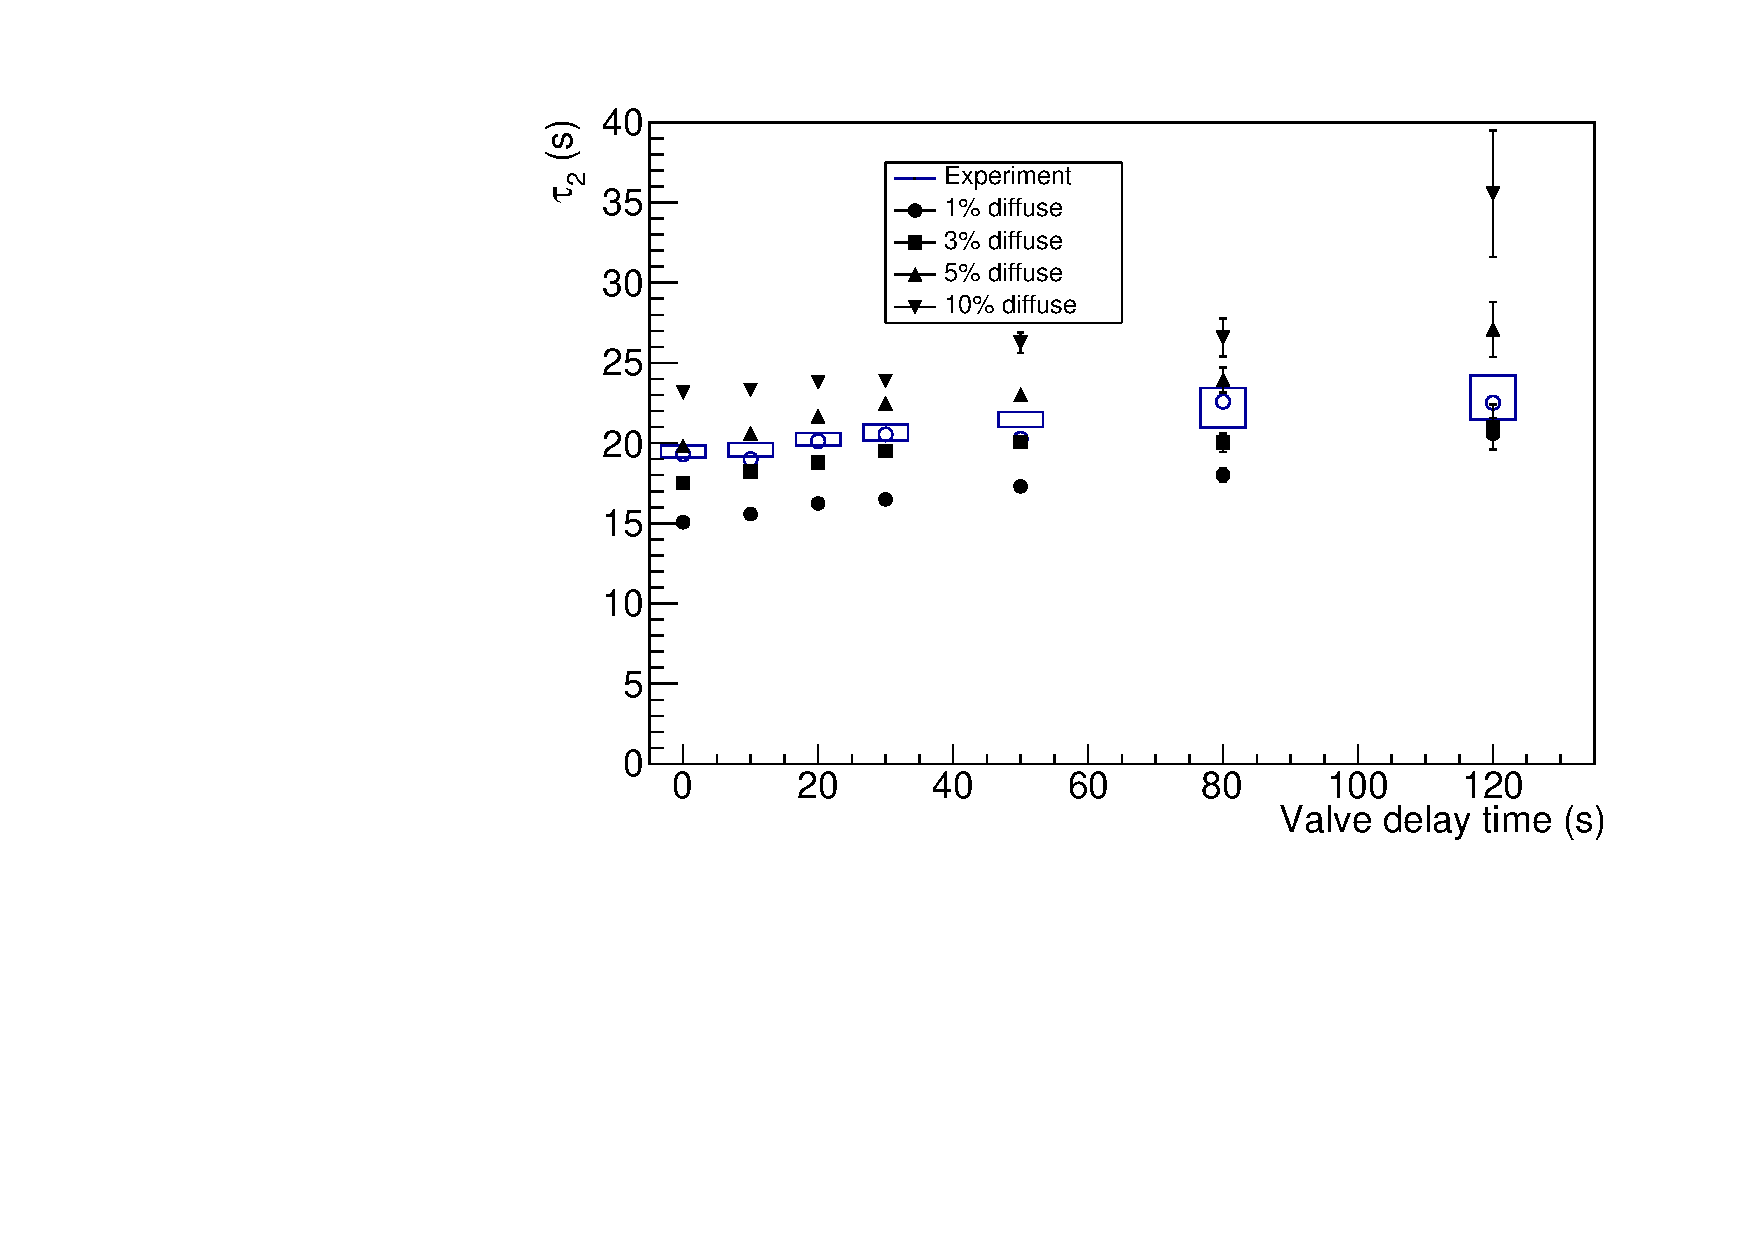
\includegraphics[width=0.9\textwidth]{falltime.pdf}
  \caption{Comparison of fall time $\tau_2$ in the experimental data
    and the simulations with different diffuse-reflection
    probabilities. The boxes indicate the second and third quartile of
    the experimental data.}
\label{fig:falltime}
%\end{figure}
%\begin{figure}[h!]
%\centering
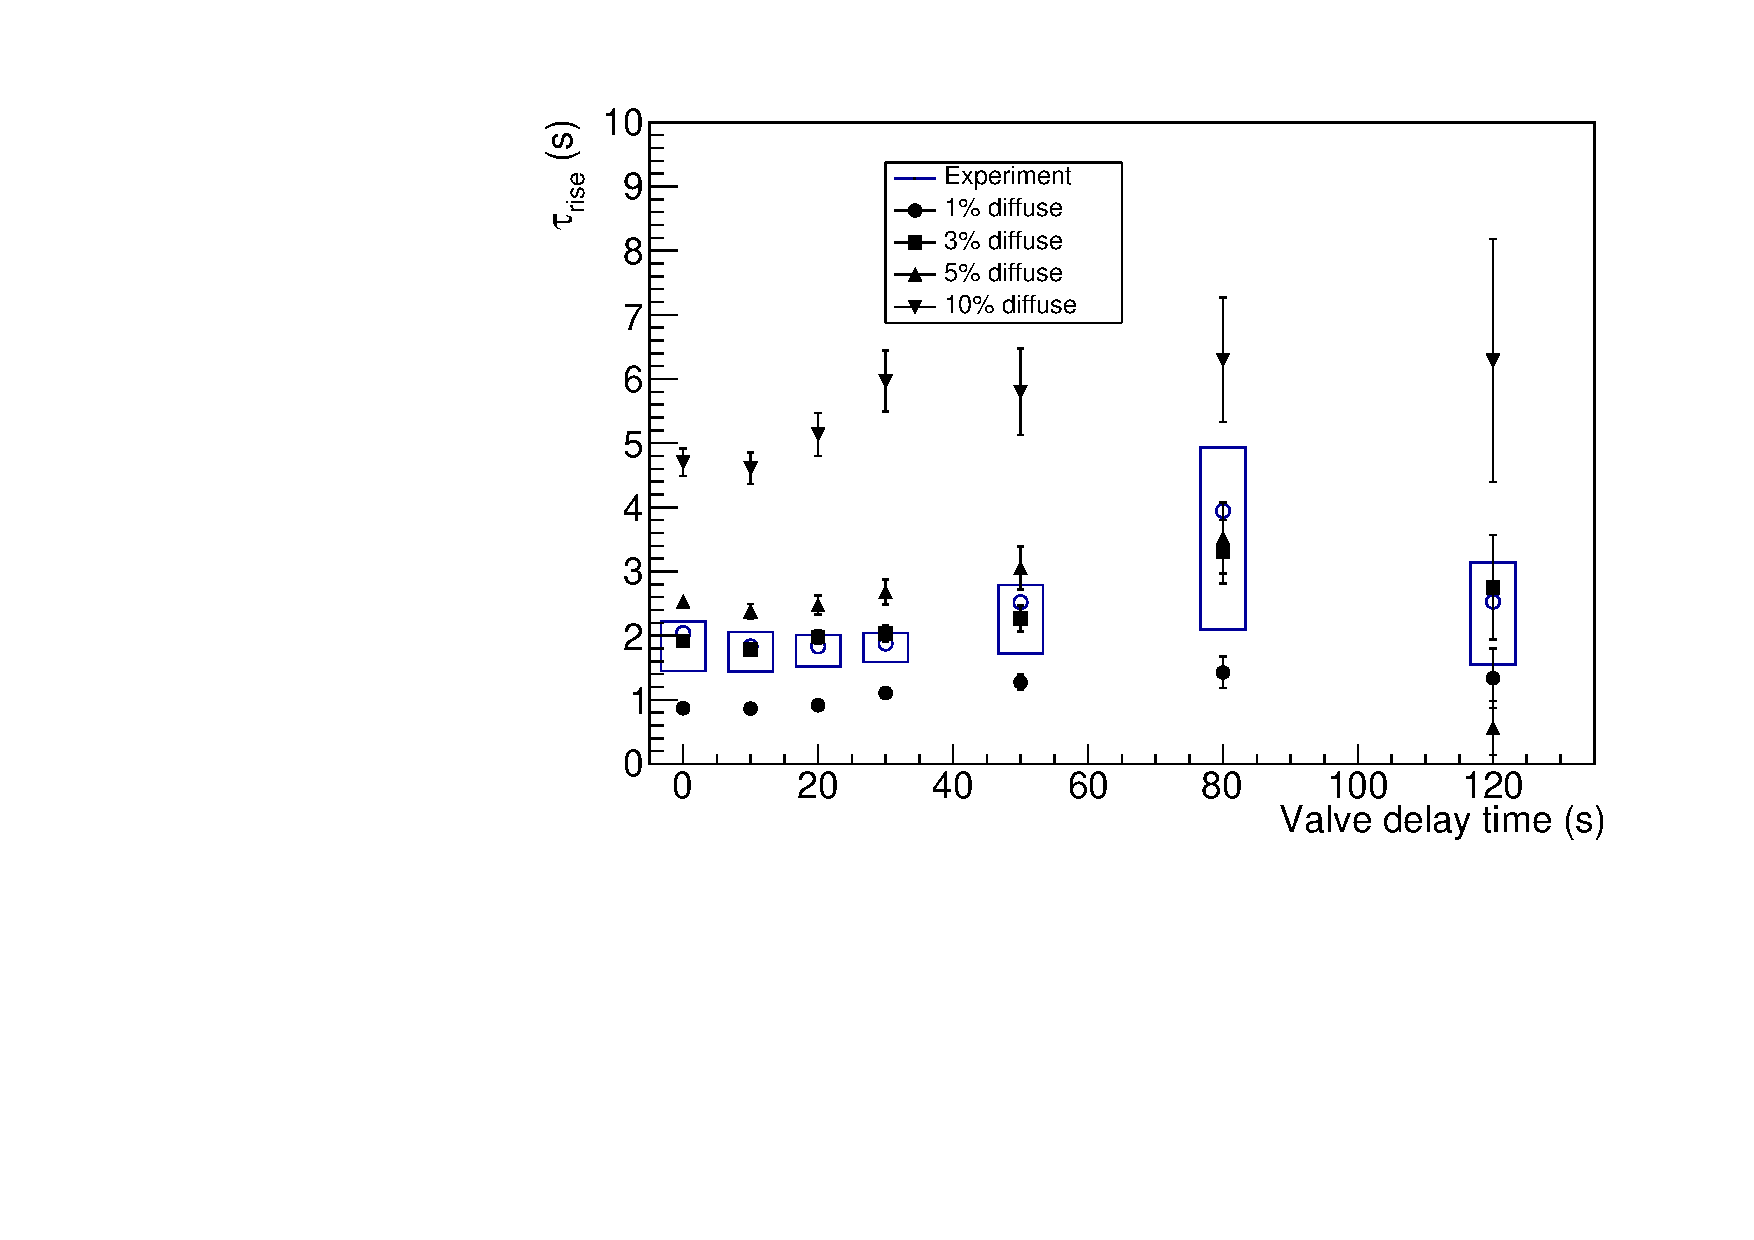
\includegraphics[width=0.9\textwidth]{risetime.pdf}
\caption{Comparison of rise time $\tau_{\mathrm{rise}}$ in
  experimental data and simulations with different diffuse-reflection
  probabilities. The boxes indicate the second and third quartile of
  the experimental data.}
\label{fig:risetime}
\end{figure}


\subsection{UCN Upscattering Coefficient}
The simulations are also used to determine the parameter
$f_{\mathrm{He}}$ or the fraction of time that UCN spends in the
superfluid helium in the detectable range of 120~neV to 200~neV.
%%%%How???
For the steady-state measurements, this fraction turned out to be
almost constant over a range of upscattering lifetime in the
superfluid helium giving

\begin{equation}
f_\mathrm{He,3} = 0.464 \pm 0.001_\mathrm{stat.} \pm 0.003_\mathrm{syst.},
\end{equation}
where the systematic uncertainty is the variation in simulations with
$\tau_{\mathrm{He}}$ from 3.05~s to 390~s. 
The Eqn.~\ref{eqn:tau2} could be rewritten as
\begin{equation}
  \label{eqn:tau2rewritten}
\tau_d^{-1} + \tau_\mathrm{wall,2}^{-1} = \tau_2^{-1}(T_0) - f_\mathrm{He,2} B \left( T_0 \right)^a
\end{equation}
where the value for $\tau_2$ is
\begin{equation}
\tau_2^{-1}(T_0) = (19.3 \pm 0.8_\mathrm{stat.})\,~\si{\second}
\end{equation}
comes from fall time in the storage lifetime measurements at the
temperature $T_0$ which is
\begin{equation}
T_0 = 0.92 \pm 0.005_\mathrm{stat.} \pm 0.05_\mathrm{syst.}.
\end{equation}
Replacing Eqn.~\ref{eqn:tau2rewritten} in Eqn.~\ref{eq:b}, $B$ can be written as
\begin{equation}
B = \frac{b \tau_2^{-1}(T_0)}{f_\mathrm{He,3} + f_\mathrm{He,2} b \left( \frac{T_0}{\SI{1}{\kelvin}} \right)^a}.
\end{equation}
Here all the parameters are known except for $ f_\mathrm{He,2}$ which
does not significantly affect the result, and hence, it is assumed to
lie between 0 and 1. As a result
\begin{equation}
B = (10.4 \pm 0.4_\mathrm{stat.} \pm 4.1_\mathrm{syst.}) \cdot 10^{-3} \, \si{\per\second}.
\end{equation}
which is consistent with the result in~\cite{Leung2016}.


%add UCN production simulation result here.


\subsection{Storage Lifetime Simulations???}



\section{Heater Tests of The Source\label{sec:heattest}}
The cooling process of the spallation neutrons create a heat input on
the cryostat including the superfluid helium. This heat input must be
removed to keep the temperature of the superfluid helium
constant. This is critical because the storage lifetime of neutrons
depend strongly to the temperature of the superfluid helium.

The heat load on the cryostat creates a temperature gradient along the
heat exchanger to the suprefluid helium bottle. The temperature
gradient in the superfluid helium is described by its heat
conductivity. The bigger the temperature difference, the lower the
heat conductivity. The temperature dependence of the heat conductivity
in the superfluid helium is describe by theorical models from the
lambda point 2.17~K down to around 1.4~K which is above the
temperature for the UCN production~($<~1$~K).  Because of the
difficulty to reach such low temperatures, the mechanism of heat
transfer in that temperature region is not fully understood.  To check
the validity of theoretical models, the extrapolation to lower
temperatures is compared to acquired data.


In order to create excess heat load on the superfluid helium, there
are heater tapes wrapped around the superfluid helium bottle. These
heaters can create a temperature gradient between the heat exchanger
and the superfluid helium bottle~(see
Sec.~\ref{sec:vertical_source}). This temperature gradient can be
measured using the temperature sensors shown in Fig.~\ref{fig:TSs}.

The heater test procedure is the following. The heater tape around the
superfluid helium bottle is turned on when the temperature of the
superfluid helium is stable. This is called the {\it{base}}
temperature. The applied heat load could easily be calculated since
the applied current and voltage are known. After the heater is turned
on, the temperature of the superfluid helium starts to increase. This
causes an increase in the flow rate in the $^3$He pot. After some time,
the temperature of the superfluid starts to settle and reach a new
equilibrium. This temperature is referred to as the
{\it{saturation}} temperature. At this point, the heater could be
turned off which causes the superfluid temperature and the flow rate
of the $^3$He to go back to the base conditions.

In 2017 two sets of heater tests were performed on the vertical UCN
source: The April heat test and the November heat test. In April the
base temperature of the superfluid helium was slightly higher than in
November. In addition, there was no proton beam during the April
cooling and it was purely a cryostat cooling
test. Table.~\ref{tab:heattest} shows the heat load and the
temperatures of those tests.

\begin{sidewaystable}
  %\centering
  \begin{tabular}{|c|c|c|c|c|c|c|c|c|c|c|}
    \hline
    Heater Power & T$_{\mathrm{base, TS10}}$ &  T$_{\mathrm{sat., TS10}}$ & T$_{\mathrm{base, TS11}}$ &  T$_{\mathrm{sat., TS11}}$ & T$_{\mathrm{base, TS12}}$ &  T$_{\mathrm{sat., TS12}}$ & T$_{\mathrm{base, TS14}}$ &  T$_{\mathrm{sat., TS14}}$ & T$_{\mathrm{base, TS16}}$ &  T$_{\mathrm{sat., TS16}}$ \\
    (mW) & (K) & (K) & (K) & (K) & (K) & (K) & (K) & (K) & (K) & (K) \\
    \hline
    \hline
    \multicolumn{11}{|c|}{\textbf{April Heat Test}}\\
    \hline
   2.5 & 0.717 & 0.718 & 0.93 & 0.931 & 0.926 & 0.9271 & 0.93 & 0.931 & 1.012 & 1.013 \\
    \hline
    12.5 & 0.717 & 0.7185 & 0.93 &  0.9315 & 0.924 & 0.929 & 0.93 & 0.9315 & 1.011 & 1.015 \\
    \hline
    25 & 0.719 & 0.723 & 0.928 & 0.931 & 0.919 & 0.929 & 0.928 & 0.931 & 1.008 & 1.015 \\
    \hline
    75 & 0.7195 & 0.7255 & 0.9285 & 0.937 & 0.922 & 0.952 & 0.928 & 0.937 & 1.01 & 1.03 \\
    \hline
    250 & 0.7175 & 0.7375 & 0.93 & 0.9475 & 0.93 & 1 & 0.93 & 0.947 & 1.01 & 1.065 \\
    \hline
    \multicolumn{11}{|c|}{\textbf{November Heat Test}}\\
    \hline
   25 & 0.724 & 0.73 & 0.892 & 0.9 & 0.84 & 0.86 & 0.92 & 0.923 & 0.96 & 0.97 \\
    \hline
    50 & 0.741 & 0.75 & 0.895 & 0.91 & 0.84 & 0.9 & 0.92 & 0.93 & 0.96 & 0.99 \\
    \hline
    75 & 0.73 & 0.74 & 0.9 & 0.91 & 0.85 & 0.92 & 0.92 & 0.93 & 0.96 & 1 \\
    \hline
    100 & 0.73 & 0.769 & 0.9 & 0.936 & 0.85 & 0.96 & 0.92 & 0.952 & 0.96 & 1.04 \\
    \hline
    150 & 0.73 & 0.755 & 0.9 & 0.93 & 0.84 & 0.99 & 0.92 & 0.945 & 0.96 & 1.06 \\
    \hline
    200 & 0.73 & 0.9 & 0.9 & 1.26 & 0.84 & 1.23 & 0.92 & 1.25 & 0.96 & 1.26 \\
    \hline
    250 & 0.73 & 0.94 & 0.895 & 1.385 & 0.84 & 1.345 & 0.92 & 1.363 & 0.97 & 1.375 \\
    \hline
  \end{tabular}
  \caption{The heater power and the base and saturation temperature of the 
    temperature sensors in the superfluid helium and in the $^3$He pot for
    the April and November heat tests.~\cite{Florian_thesis}}
  \label{tab:heattest}
\end{sidewaystable}


\subsubsection{Theoretical Models}
The relationship between the heat flux and the temperature gradient in
a one dimentional channel is written as following

\begin{equation}
  \label{eq:q_dT}
  q^m = f^{-1}\left(T, p \right) \frac{dT}{dx}
\end{equation}
Where $q$ is the input heat flux, $T$ is the temperature, $p$ is the
pressure and $\frac{dT}{dx}$ is the temperature gradient along the
channel and $f\left(T, p \right)$ is the heat conductivity fucntion
which controls the temperature gradient of the heat flux and could be
written as
\begin{equation}
  \label{eq:f}
f \left( T, p \right) = \frac{A_\mathrm{GM}\rho_n}{\rho_s^{3}s^4T^3}
\end{equation}
where $\rho_n$ is the density of the normal fluid component, $\rho_s$
is the density of the superfluid component, $s$ is the specific
entropy, $T$ is the temperature and $A_\mathrm{GM}$ is the
Gorter-Mellink parameters which describes the friction between the
normal fluid component and the superfluid component.

Since the Gorter-Mellink parameter is not known, he calculation of
$f \left( T, p \right)$ in the form of Eq.~\ref{eq:f} is difficult
because. However, there are other models to describe the behaviour of
the heat conductivity functions. There are two models that are
considered here at the saturated vapour pressure. As a result, the
pressure dependence could be neglected. The models are the theory
model from Van Sciver~\cite{van2012helium} and the HEPAK
model~\cite{arp2005hepak}. Fig.~\ref{fig:VanSciver_vs_HEPAK}

\begin{figure}[h!]
  \centering 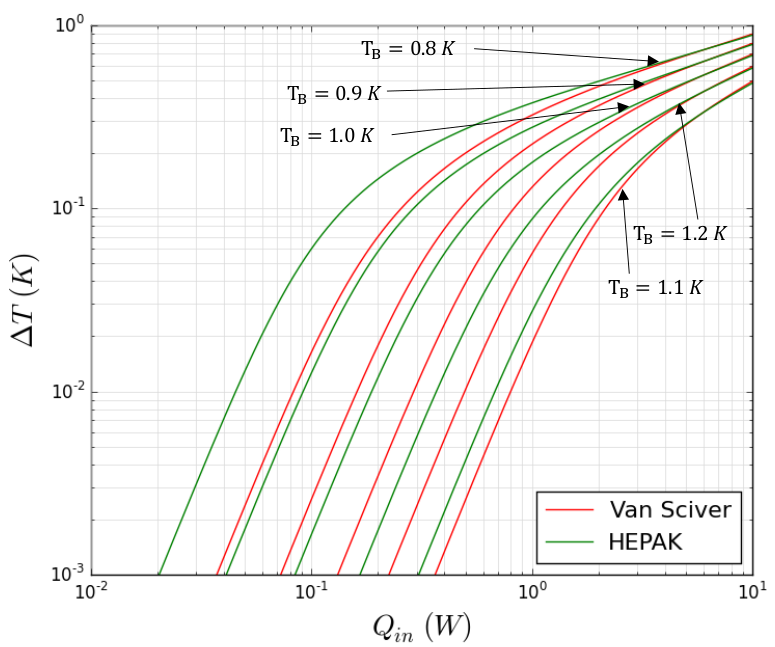
\includegraphics[width=0.8\textwidth]{VanSciver_vs_HEPAK.png}
  \caption{The heat conductivity function of the Van Sciver and HEPAK
    models. The vertical axis shows the temperature gradiant along the
    channel and the horizonal axis shows the input heat
    flux~\cite{Florian_thesis}. The arrows on the graph indicate the
    temperature of the superfluid helium}
\label{fig:VanSciver_vs_HEPAK}
\end{figure}

As Fig.~\ref{fig:VanSciver_vs_HEPAK} shows, at higher heat input both
models tend to agree. However, at lower heat inputs, the heat
conductivity function values for the Van Sciver model lie below the
values for the HEPAK model. In addition, as the temperature of the
superfluid helium increases, the heat conductivity function tends to
look more linear. Since the Van Sciver model is more well known, it is
used for comparision with experimental data.

\subsubsection{Measurement Result}
The data shown in Table.~\ref{tab:heattest} is a set of cleaned data
from all the heat tests in 2017. If the heat load on the cryostat is
higher than its cooling power, the temperature of the superfluid
helium would increase linearly without reaching an equilibrium. This
phenomena has been observed for higher heater powers e.g. 1~W. As a
result, that data is discarded.


Fig.~\ref{fig:April_Data} shows the result of the April heat test.
For a given heat input, the temperature difference between the base
and the saturation temperature for each temperature sensor is
calculated~(see table~\ref{tab:heattest}). The average of all of those
temperature differences give the overall $\Delta T$ across the
channel. Those are shown with black dots in Fig.~\ref{fig:April_Data}
as the raw data. However, the heat input for each data point should be
corrected since the total heat input is a combination of the added
heat from the heater tapes and the background heat load on the
cryostat which is not taken into account.


\begin{figure}[h!]
  \centering 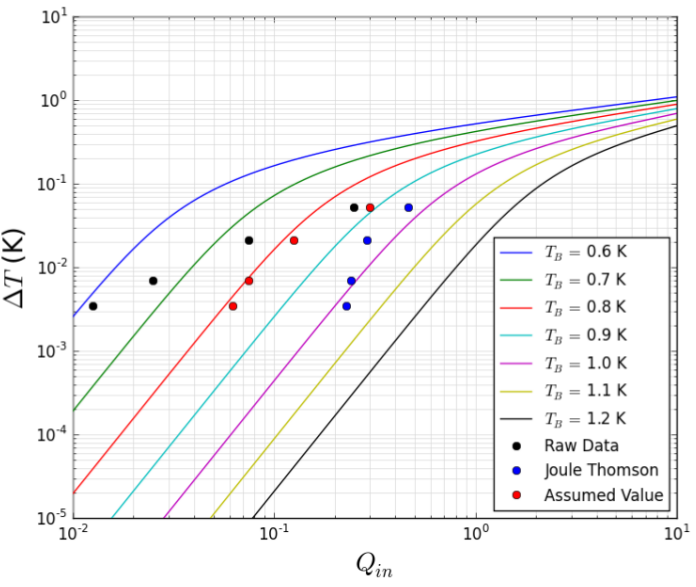
\includegraphics[width=0.8\textwidth]{April_Data.png}
  \caption{The comparison between the April heat test data and the Van
    Sciver model. The lines show the Van Sciver model's heat
    conductivity function at different superfluid helium bath
    temperatures. The black data points show the measured raw data of
    the heat tests. The blue points are the Joule Thomson values,
    which are the raw data plus the calculated background heat
    (included Joule-Thomson effect) and the red points show the raw
    data with the assumed 50 mW background heat input. }
\label{fig:April_Data}
\end{figure}


The two other sources of heat input to be considered are the
Joule-Thomson expansion and the the background heat load to the $^3$He
pot due to the thermal readiation and to the superfluid helium
bottle. The Joule-Thomson expansion happens when a gas or liquid
passes through a valve which has different temperature and pressures
on both sides while there is no heat exchange to the environment. Here
$^3$He flows into the heat exchanger and passes through a valve with
different pressures and temperatures on two sides. Because of the
Joule-Thomson expansion some liquid changes into vapor which is then
directly pumped out of the system and does not contribute to the
cooling process. For the backround heat load, based on estimations of
the sources of the background heat to the bottle alone, combined with
the measurements of the mass flow of $^4$He from the top of the bottle
when the $^3$He system is switched off, a heat of $\simeq$~50~mW is a
reasonable estimate of the true background heat to the bottle
alone. In Fig.~\ref{fig:April_Data}, the assumed values are the sum of
the 50~mW background heat and the heat input from the heaters and the
Joule-Thomson values are the sum of the heat input from the heaters
plus the calculated 232~mW calculated background
heat~\cite{Florian_thesis}.



Fig.~\ref{fig:November_Data} shows the data with the heaters in
November as well as the theoretical model of Van Sciver for the heat
conductivity. Each color represents a temperature range. The markers
are the actual data taken in November 2017.

At all the temperture ranges, the acquired data shows lower heat load
compared to the theoretical model. At the range of 1.2-1.3~K, the data
point with the smaller $\Delta$T is acquired at a higher He-II base
temperature, whereas the data point with higher $\Delta$T is acquired
at standard He-II base temperature. The data points which are closer
to the theoretical models are acquired at lower base temperature for
the superfluid helium. Since the measured data show bigger temperature
differences compared to the theoretical model of Van Sciver, it
suggests that the theory is assuming higher heat conductivity. Looking
back at Fig.~\ref{fig:VanSciver_vs_HEPAK}, it shows that using the
HEPAK model might solve this problem since the HEPAK model shows lower
heat conductivity.

One reason between the disagreement between the measurements and
theory could be the fact that these theoretical models are only
measured down to 1.4~K and they are extrapolated to lower
temperatures. Another reason could lie in the geometry difference. The
theoretical models are valid for a one-dimensional channel while there
is a 90$^\circ$ bend in the experimental setup~(see
Fig.~\ref{what???}) which can cause a higher temperature differnece
across the channel. One other reason might be the uncertainty in the
measured temperature due to the calibration of the temperature
sesnors. There might be other unknown sources of systematic error
affecting the measurements.


\begin{figure}[h!]
  \centering 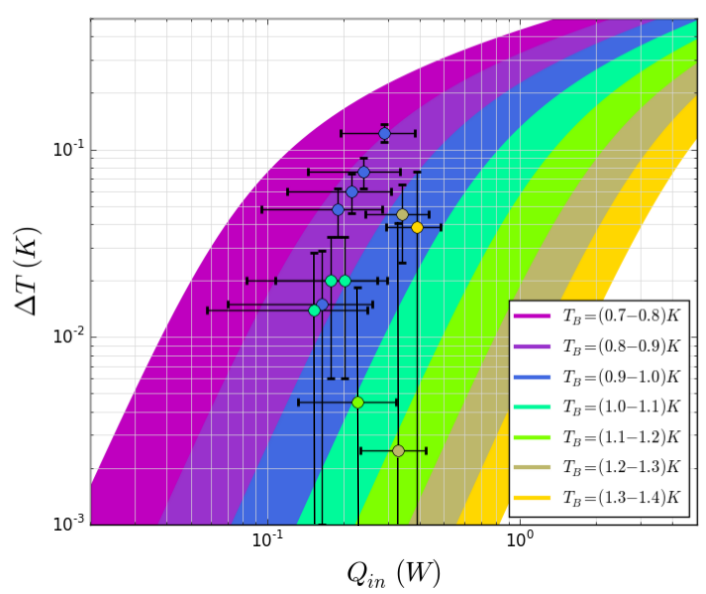
\includegraphics[width=0.8\textwidth]{November_Data.png}
  \caption{Theoretical model of Van Sciver for the heat conductivity
    at different temperature ranges and the November data. The
    vertical axis shows the temperature difference between the base
    and the saturation temperature for temperature sensors. The
    horizontal axis shows the heat input from the heaters plus the
    background heat.}
\label{fig:November_Data}
\end{figure}

\subsection{Heater Test Versus Proton Beam Current}
One of the UCN experiments was designed to match the heater power from
the heaters wrapped around the UCN bottle with the proton beam
current.

The result of the heater tests were disscused in
Section~\ref{sec:heattest}. The application of the heat on the
superfluid helium bottle gives rise to a temperature increase in the
superfluid helium as well as a flow rate increase in the $^3$He
pot. The amount of this heat load is known simply by knowing the the
applied current to the heater tapes. However the input heat load is
not known in the case of the target irradiation. As a result, the
steady-state UCN yield were measured at different proton beam
current. The target irradiation at higher beam currents give rise to a
temperature change in the superfluid helium. In addition, the increase
in the heat load increases the $^3$He flow rate in the $^3$He pot.
The comparison of the temperature and flow rate increase between these
experiments give an idea of the amount of applied heat load on the
superfluid helium bottle for each given proton beam current.

Even though the result of the data analysis for this experiment was
not conclusive, it gave an idea of the stability and the behaviour of
the helium cryostat and a better experimental plan for the future.

Some unexpected anomalies were observed during the measurement. For
instance, when the 4~K resorvior was being filled, the flow rate in
the $^3$He pot as well as the temperature in the superfluid helium was
not stable. Another problem arose from the wait time between the
measurements. Before conducting a new measurement, it is essential to
wait long enough so that the superfluid helium temperature and $^3$He
flow rate go down to a stable value. In some cases, the wait time
between the measurements was not long enough and so the it was not
possible to assign a change in the superfluid helium temperature or
$^3$He flow rate. In addition, target irradiation should be long
enough so that the temperature and the $^3$He flow rate reach a stable
value.

Fig.~\ref{fig:problemrun} shows an inconclusive run. The top graph
shows the UCN rate over time. This shows an increase in the UCN rate
after starting the target irradiation. At the end of the irraidation,
the UCN rate decays to the typical background rate. The middle graph
shows the temprature of the superfluid helium from the temprature
sensor TS12 over time. Here the irradiation of the target stopped
before the superfluid helium could reach a stable saturation
value. The bottom graph shows the flow rate in the $^3$He from the
sensor FM1~(see Fig.~\ref{fig:gasflow}). At the beginning of the run,
the flow rate was still going down and it did not reach a minimum
stable value. Typically this value was around 14~SLM. In addition, the
flow rate did not reach a maximum saturation value due to short target
irradiation time. Therefore, the change in the flow rate is not
inclusively due to the teraget irradiaton and is not conclusive.



\begin{figure}[h!]
  \centering 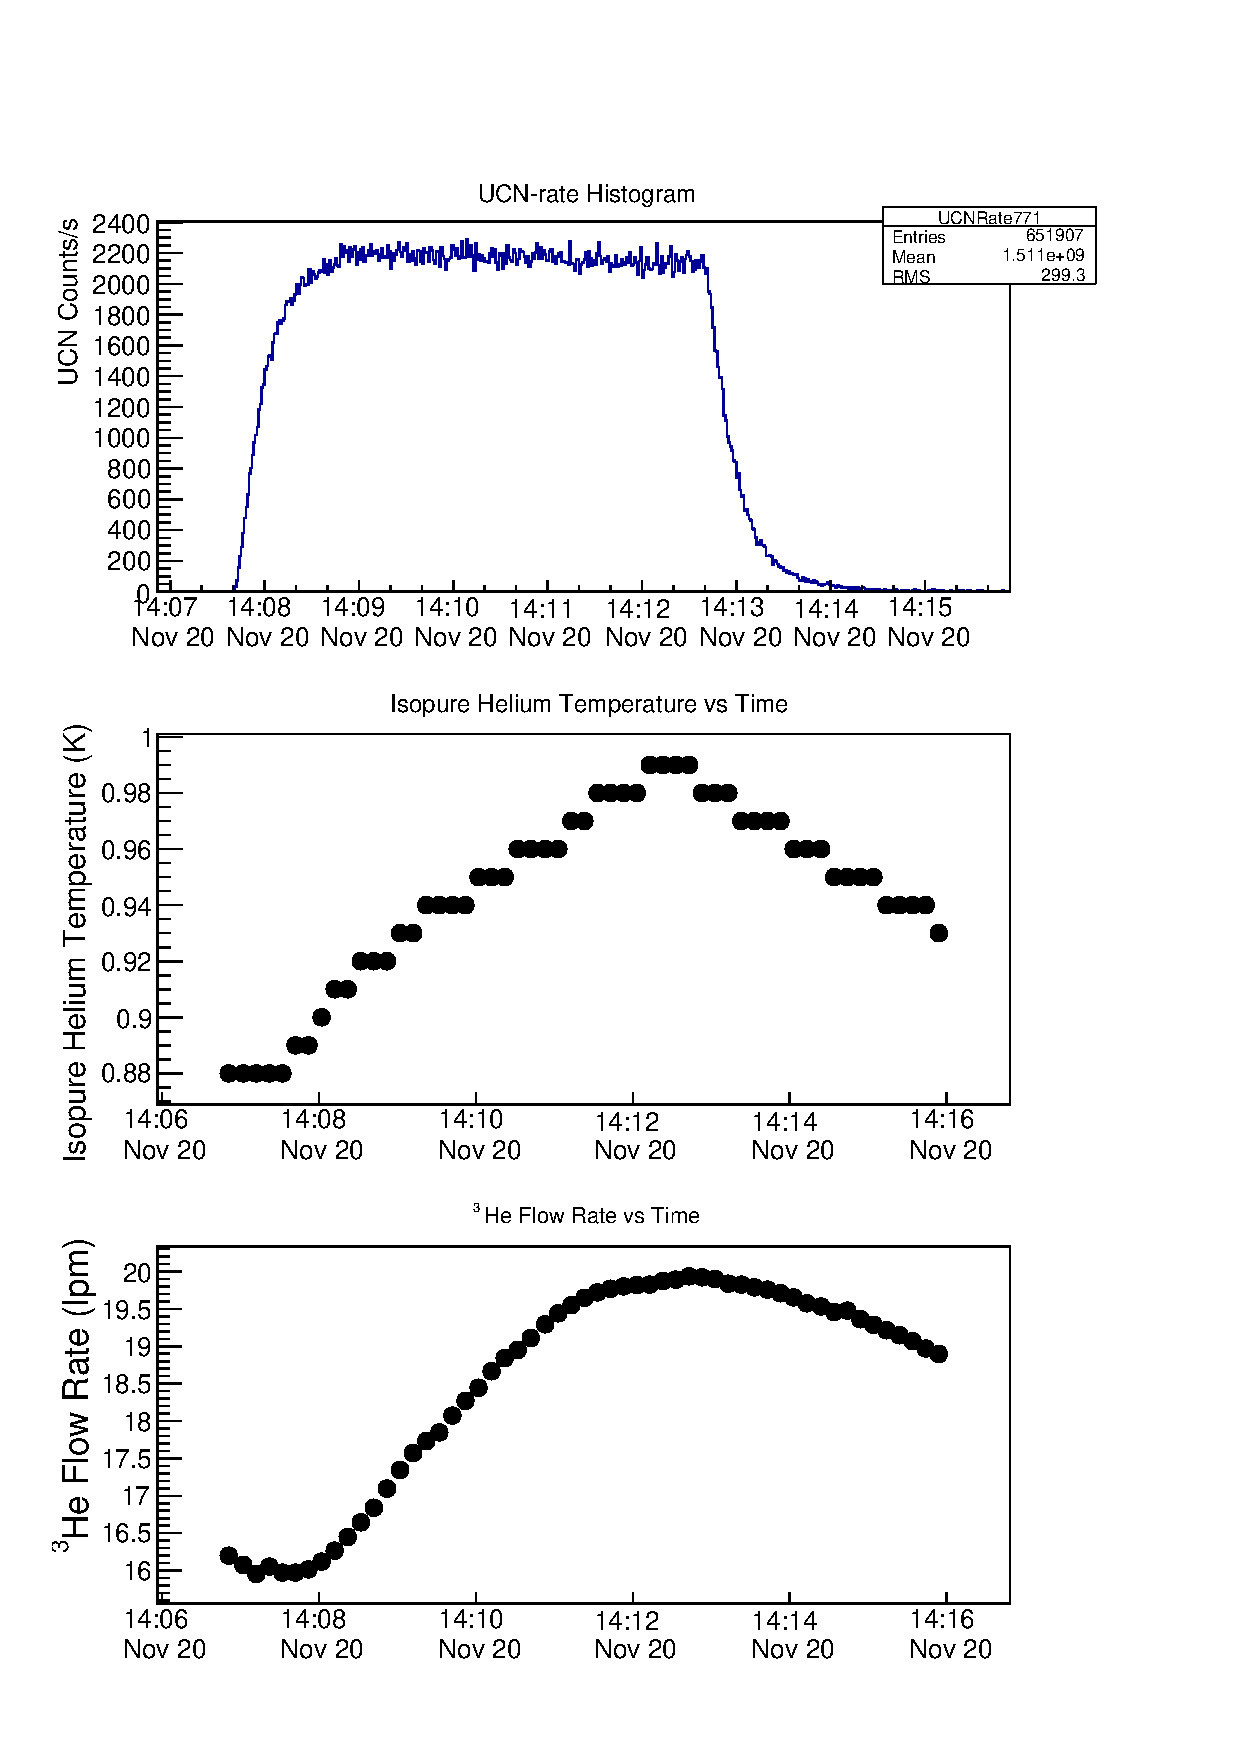
\includegraphics[width=0.8\textwidth]{problemrun.pdf}
  \caption{Steady-state UCN production data for 1.5~$\mu$A proton beam
    current. The top graph shows the UCN rate over time, the middle
    graph shows the superfluid helium temperature~(TS12) over time and
    the bottom graph shows the $^3$He flow rate versus time. Detail
    provided in text.}
\label{fig:problemrun}
\end{figure}


\section{Summary}

The result of the first UCN production with the vertical UCN source at
TRIUMF were discussed. The measurements include the UCN yield
experiments, UCN storage lifetime experiments and steady-state UCN
production experiments.

The maximum number of UCN achieved for the standard 1~$\mu$A proton
beam current at 60~s target irradiation was 40000 and the highest
number of UCN counts was 325000 at 10~$\mu$A beam current and 60~s
irradiation of the target.  The experimental period took about two
weeks. In this time, the storage lifetime of UCN decreased from 37~s
to 27~s with about 2~\% decrease per day due to the source
contamination after openning the UCN valve. The UCN counts also showed
a decrease of about 40~\% due to the source contamination as well as
different experimental configuration at later dates. The steady-state
UCN rate showed to be around 1600~UCN/s/$\mu$A.

To decrease the temperature of the superfluid by 0.1~K a 5~min wait
between the cycles is necessary. It is also concluded that, if
interested in the $^3$He flow rate, the data acquisition should happen
after the 4~K reservoir filling.





\UCNreport{Detector Comparison\label{sec:detector_comparison}}
Using the rotary valve

%\section{Background Measurements}
%With Ni foil

%\section{UCN guide Transmission Measurements}

%\section{Result And Conclusion}

%\begin{description}
%\item{I think this belongs to this chapter: UCN production by
%  multiphonon excitation in superfluid helium (I can use my candidacy
%  report for this part as a start)}
  
%\item{Some information about the detector}
  
%\item{UCN data goes here}
  
%\item{what else?}
%\end{description}
